
\chapter{Learning from Wizard-of-Oz data}
\label{chap:wozlearning}

%\note{IN CONSTRUCTION - NOT READY YET }

The previous chapter outlined the formalism of probabilistic rules and described how these rules are instantiated at runtime to update the dialogue state and perform action selection. Probabilistic rules are associated to a number of parameters, which may either express probabilities over effects (for probability rules) or utilities associated with particular decisions (for utility rules). But where do these probabilities and utilities exactly come from?

We have developed in this thesis two distinct approaches to this question. The present chapter concentrates on the first approach, which is based on supervised learning techniques. We demonstrate how rule parameters can be optimised to best imitate the decision choices of an human expert through a process of statistical estimation on Wizard-of-Oz data. The next chapter will then detail an alternative, reinforcement learning approach to the same task.

The chapter is divided in three sections.  Section \ref{sec:rule-params} describes how uncertainty regarding the value of rule parameters can be explicitly represented through prior distributions. Section \ref{sec:rule-supervised} spells out how these distributions can be gradually refined through Bayesian learning on data gathered from Wizard-of-Oz interactions.  The learning algorithm  is used to progressively narrow down the spread of the parameter distributions to the values providing the best fit for the training data. Finally, Section \ref{sec:wozlearning-experiments} presents experimental results in a human-robot interaction domain for which small amounts of Wizard-of-Oz data were recorded. The experiment compared the learning performance of a utility model structured with probabilistic rules against two baselines respectively encoded with plain utility tables and with linear models. The evaluation showed that the rule-structured model was able to imitate the wizard policy significantly better than its unstructured counterparts.

\section{Parameters of probabilistic rules}
\label{sec:rule-params}

\subsection{Generalities}

The examples of probabilistic rules analysed so far all relied on fixed probability and utility values. These values can however be replaced by parameters that reflect unknown values that are to be estimated empirically, on the basis of training data. 
 
The learning methods developed in this thesis focus on the problem of parameter estimation given a known rule structure.  Although some structure learning approaches have been developed in the literature on statistical relational learning \citep[see e.g. ][]{PasulaZK07,Kok:2009}, they are generally confined to domains of limited size and full observability. We assume in this thesis that the \textit{if ... then ... else} structures of probabilistic rules are best defined by the system designer, while the effect parameters can be estimated via statistical techniques. Based on our own practical experience with various dialogue systems, we believe that such division of labour between the human designer and the learning algorithm is a sensible one, as system designers generally have a good grasp of the domain structure and relations between variables, but are often unable to quantify the precise probability of an effect or utility of an action.\footnote{Humans are indeed notoriously poor at estimating probabilities and are prone to multiple cognitive biases, as evidenced by numerous studies in behavioural psychology.  The interested reader is invited to consult e.g. \cite{KahnemanSlovicTversky81,morganhenrion} for more details on the psychological aspects of the human perception of uncertainty and the difficult problem of probability elicitation from experts.}

The overall structure of parametrised rules remains essentially identical to the one outlined in Section \ref{sec:formalisation}.  Parametrised probability rules continues to be defined in terms of conditions $c_i$ associated to probability distributions $P(E_i)$ over possible effects.  The probability of each effect $e_i^j$ is however no longer fixed but is represented by a parameter $\theta_{(i,j)}$, giving rise to the following rule skeleton: 
\begin{equation}
\begin{aligned}
& \textbf{if} \ \ (c_{1}) \ \ \textbf{then} \\ 
& \;\;\;\;\; \begin{cases}
P(E_1\!=\!e_1^1) = \theta_{(1,1)} \\
 ... \\
P(E_1\!=\!e_1^{m_1}) = \theta_{(1,m_1)} 
\end{cases} \\[3mm]
%& \textbf{else if} \ \ (c_{2}) \ \ \textbf{then} \\ 
%& \;\;\;\;\; \begin{cases}
%P(E_2\!=\!e_2^1) = \theta_{(2,1)}, \\
% ... \\
%P(E_2\!=\!e_2^{m_2}) = \theta_{(2,m_2)}
%\end{cases} \\ 
& ...  \\
& \textbf{else} \\
& \;\;\;\;\; \begin{cases}
P(E_{n}\!=\!e_{n}^1) = \theta_{(n,1)} \\
... \\
P(E_{n}\!=\!e_{n}^{m_{n}}) = \theta_{(n,m_n)}
\end{cases}
\end{aligned}
\label{eq:probrule}
\end{equation}

The notation $\theta_{(i,j)}$ express the parameter associated with condition $i$ and effect $j$.  The $\boldsymbol\theta$ parameters must satisfy the axiomatic constraints $\theta_{(i,j)} \geq 0  \ \forall i,j$ and $\sum_{j = 1}^{m_i} \theta_{(i,j)} = 1 \ \forall i$.

Parametrised utility rules are expressed similarly by replacing fixed utility values with unknown parameters:
\begin{equation}
\begin{aligned}
& \textbf{if} \ \ (c_{1}) \ \ \textbf{then} \\ 
& \;\;\;\;\; \begin{cases}
U_1(d_1^1) = \theta_{(1,1)} \\
 ... \\
U_1(d_1^{m_1}) = \theta_{(1,m_1)}
\end{cases} \\[3mm]
%& \textbf{else if} \ \ (c_{2}) \ \ \textbf{then} \\ 
%& \;\;\;\;\; \begin{cases}
%U_2(d_2^1) = \theta_{r(2,1)} \\
% ... \\
%U_2(d_2^{m_2}) = \theta_{r(2,m_2)}
%\end{cases} \\
& ...  \\
& \textbf{else} \\
& \;\;\;\;\; \begin{cases}
U_n(d_n^1) = \theta_{r(n,1)} \\
... \\
U_n(d_n^{m_n}) = \theta_{r(n,m_n)}
\end{cases}
\end{aligned}
\end{equation} \\

Domain models can be composed of both fixed and parametrised rules and can therefore accommodate a wide spectrum of learning tasks from fully statistical models with virtually no prior knowledge to manually designed models with only a handful of parameters. 

\subsection{Parameter priors}
\label{sec:rule-params-priors}

We adopt in this thesis a Bayesian approach to parameter estimation and associate the rule parameters with explicit prior distributions over their range of possible values.  The benefits of Bayesian approaches compared to traditional maximum likelihood methods are multiple:
\begin{enumerate} 
\item Bayesian methods allow domain knowledge to be included into the learning cycle through the use of informative priors (cf. discussion below). The system designer is thus free to bias the initial prior distributions according to her/his domain expertise.
\item Bayesian methods explicitly capture the model uncertainty before and after learning.  The outputs of a Bayesian learning experiment are indeed full posterior distributions over the possible parameter values instead of being reduced to point estimates (as for maximum likelihood estimation).  The dialogue agent can therefore explicitly account for this parameter uncertainty at runtime and use it to simultaneously learn, reason and act in its environment \citep{Ross:2011}. Furthermore, the reliance on full parameter distributions facilitates the combination of multiple learning processes, as the posterior distribution generated by one learner can be passed on as the prior distribution of another. 
\end{enumerate}

Prior parameter distributions generally have a continuous range, but their exact shape depends on the type of parameter they seek to encode. We first review parameters of probability distributions and then discuss possible parameter priors for utility values.  Appendix \ref{chap:probdistributions} provides more detail on the mathematical properties associated with these distributions.

\subsubsection*{Probability parameters}

That the distributions over the effects of probability rules are defined as categorical probability distributions.  As discussed in Section \ref{sec:learning}, the parameter priors of categorical distributions are best expressed via \textit{Dirichlet} distributions. 

Each distribution over effects $P(E_i)$ is defined by its own Dirichlet distribution of dimension $m_i$, where $m_i$ is the number of alternative effects (including the empty effect if appropriate).  Rule $r_{1}'$ provides an example of probability rule adapted from $r_1$ (cf. previous chapter) with the fixed probabilities replaced by Dirichlet parameters:
\begin{align*}
r_{1}: \ \ \ \ \ & \textbf{if} \ (\mathit{Rain}\!=\!\mathit{false} \land \mathit{Weather}\!=\!\mathit{hot}) \ \textbf{then} \\
& \;\;\;\;\;  \begin{cases}
 P(\mathit{Fire}\!=\!\mathit{true}) = \theta_{r_{1}(1,1)} \\ 
P(\mathit{Fire}\!=\!\mathit{false}) = \theta_{r_{1}(1,2)}
\end{cases} \\ 
& \textbf{else} \\
& \;\;\;\;\; \begin{cases}
P(\mathit{Fire}\!=\!\mathit{true}) = \theta_{r_{1}(2,1)} \\
P(\mathit{Fire}\!=\!\mathit{false}) = \theta_{r_{1}(2,2)}
\end{cases} 
\end{align*}


Rule $r_{1}$ makes use of two Dirichlet distributions $P(\boldsymbol\theta_{r_{1}(1)})$ and $P(\boldsymbol\theta_{r_{1}(2)})$ respectively associated with the effect distributions for the first and second condition.  The Dirichlet distributions in this example each have two dimensions since two alternative effects are mentioned in the rule. 

Dirichlet distributions are continuous, multivariate distributions defined by the meta-parameters $\boldsymbol\alpha = [\alpha_1,... \alpha_k]$, where $k$ corresponds to the dimensionality of the categorical distribution of interest.  Dirichlet distributions over the parameters $\theta_1,... \theta_k$ are formally defined by the following probability density function:
\begin{align}
P(\theta_1,...\theta_k) = \frac{1}{\mathrm{B}(\boldsymbol\alpha)} \prod_{i=1}^k \theta_i^{\alpha_i - 1} \ \ \ \text{where } \mathrm{B}(\boldsymbol\alpha) = \frac{\prod_{i=1}^k \Gamma(\alpha_i)}{\Gamma\bigl(\sum_{i=1}^k \alpha_i\bigr)}
\end{align}

with $\Gamma$ denoting the gamma function.\footnote{The gamma function is a generalisation of the factorial for real numbers, and is defined as $\Gamma(z) = \int_0^\infty  t^{z-1} e^{-t}\,{\rm d}t$.}

Figure \ref{fig:dirichletfun} shows the shape of the probability density function for a two-dimensional Dirichlet distribution $P(\theta_1,\theta_2)$, which is equivalent to a \textit{Beta} distribution. The value for the second dimension $\theta_2$ is not explicitly shown on the figure but can be directly derived from the first value, since $\theta_1 + \theta_2=1$.  We can observe how the hyper-parameters $\boldsymbol\alpha$ determine the shape of the distribution. As the $\boldsymbol\alpha$ counts grow larger, the probability density function becomes increasingly focused on a particular region of the parameter space.  The $\boldsymbol\alpha$ counts can therefore be tuned to skew the distribution in a particular direction based on prior domain knowledge. Such prior distributions are called ``informative'' priors, since their shape is influenced by expert information. In the absence of such information, non-informative Dirichlet distributions such as $\mathrm{Dirichlet}(1,1)$ can also be used. 

\begin{figure}[h]
\centering
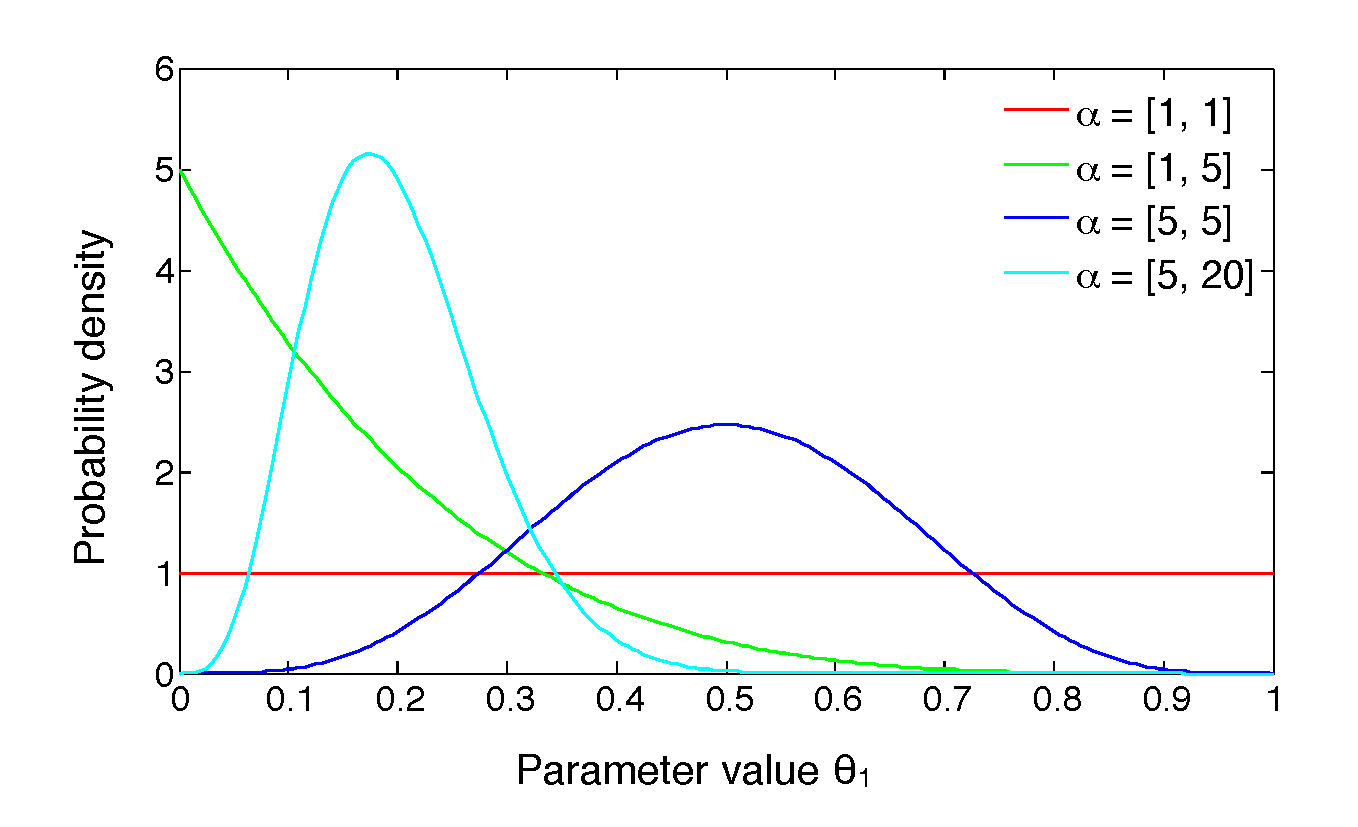
\includegraphics[scale=0.4]{imgs/dirichletfun.pdf}
\caption{Probability density functions for the Dirichlet distribution $P(\theta_1, \theta_2)$  with various values for the $\boldsymbol\alpha$ hyper-parameters.}
\label{fig:dirichletfun}
\end{figure}

As Dirichlet distributions are conjugate priors of categorical distributions, their posterior distribution after the observation of an effect remains a Dirichlet distribution with updated counts. For instance, the posterior distribution of $\boldsymbol\theta_{r_{1}(1)}$ after observing a fire when $\mathit{Rain}\!=\!\mathit{false} \land \mathit{Weather}\!=\!\mathit{hot}$ can be derived from Bayes' rule: 
\begin{align}
&P(\boldsymbol\theta_{r_{1}(1)} \; | \; \mathit{Fire}\!=\!\mathit{true}, \mathit{Rain}\!=\!\mathit{false}, \mathit{Weather}\!=\!\mathit{hot}) \nonumber \\
& = \eta \ P(\mathit{Fire}\!=\!\mathit{true} \; | \; \mathit{Rain}\!=\!\mathit{false}, \mathit{Weather}\!=\!\mathit{hot}, \boldsymbol\theta_{r_{1}(1)}) \ P(\boldsymbol\theta_{r_{1}(1)}) \nonumber \\
& = \eta \ \theta_{r_{1}[1,1]} \ \mathrm{Dirichlet}(\alpha_1,\alpha_2) \nonumber \\
& = \eta' \ \theta_{r_{1}(1,1)} \ \prod_{i=1}^2 \theta_{r_{1}(1,i)}^{\alpha_i - 1}   = \eta' \ \textrm{Dirichlet}(\alpha_1+1,\alpha_2) \nonumber
\end{align}
where $\eta, \eta'$ are normalisation factors.  Given a prior distribution $P(\boldsymbol\theta_{r_{1}(1)}) \sim \mathrm{Dirichlet}(\alpha_1, \alpha_2)$, the posterior distribution for $\boldsymbol\theta_{r_{1}(1)}$ after the observation  $\mathit{Fire}\!=\!\mathit{true}$ is thus another Dirichlet distribution $\sim \mathrm{Dirichlet}(\alpha_1+1,\alpha_2)$. 

%$For instance, we can encode the fact that the user is unlikely to change his intention after a clarification request by assigning a higher $\alpha$ value to the intention $i_u'$ corresponding to the current value $i_u$ when $a_m$ is a clarification request. 


\subsubsection*{Utility parameters}

The parameters of utility rules are also described by probability density functions.  However, contrary to probability values, the values in a utility distribution are independent of one another and are not subject to range constraints. Each utility value $u_i^j$ assigned to decision $d_i^j$ is therefore associated with its own, univariate distribution.

Rule $r_{2}$ illustrates a utility rule with four independent parameters:
\begin{align*}
r_{2}: \ \ & \textbf{if} \ (\mathit{Fire}\!=\!\mathit{true}) \ \textbf{then} \\
& \;\;\;\;\;  \begin{cases}
U(\mathit{Tanker}\!=\!\mathit{drop\mbox{-}water}) = \theta_{r_{2}(1,1)} \\
U(\mathit{Tanker}\!=\!\mathit{wait}) = \theta_{r_{2}(1,2)}
\end{cases} \\
& \textbf{else} \\
& \;\;\;\;\; \begin{cases}
U (\mathit{Tanker}\!=\!\mathit{drop\mbox{-}water}) = \theta_{r_{2}(2,1)} \\
U(\mathit{Tanker}\!=\!\mathit{wait}) = \theta_{r_{2}(c_2)-2}
\end{cases}
\end{align*}

Several types of density functions can be applied to define the prior distributions over these utility values.  We focused in this thesis on two specific families of priors, one non-informative (uniform distributions) and one informative (normal distributions): 
\begin{enumerate}
\item Continuous uniform distributions are defined on an interval $[a,b]$ with the following probability density function: 
\begin{equation}
P(\theta) = \begin{cases}
\frac{1}{b - a} & \text{for } \theta \in [a,b]  \\
0               & \text{otherwise}
\end{cases}
\end{equation}
For utility distributions, the interval $[a,b]$ corresponds to the allowed range of utility values for the domain.

\item Normal (also called Gaussian) distributions are defined by a probability density function revolving around a mean $\mu$ and variance $\sigma^2$:
\begin{equation}
P(\theta) = \frac{1}{\sqrt{2\pi\sigma^2}}\operatorname{exp}\left\{-\frac{\left(\theta-\mu\right)^2}{2\sigma^2}\right\}
\end{equation}
The range of possible values can be further constrained by truncating the density function.

\end{enumerate}

Normal distributions are well suited to represent utility values for which rough initial estimates are available. If a particular utility value can be assumed to revolve around a certain value $\tilde{u}$, its probability distribution $P(\theta)$ can be expressed via a normal distribution with a mean $\tilde{u}$ and a variance reflecting the confidence in the provided estimate. 

Figure \ref{fig:uniformn} illustrates three instances of probability density functions for a parameter $\theta$.  The first distribution corresponds to a uniform distribution on the interval $[-2,4]$, while the second is a normal distribution with mean $\mu=2$ and variance $\sigma^2=4$, and the third another normal distribution  with mean $\mu=2$ and variance $\sigma^2=1$ .  The normal distributions illustrate how prior knowledge about the utility value can be incorporated in the prior -- in this case, the distributions rest on the assumption that the true utility value is likely to revolve around the value 2. 

\begin{figure}[h]
\centering
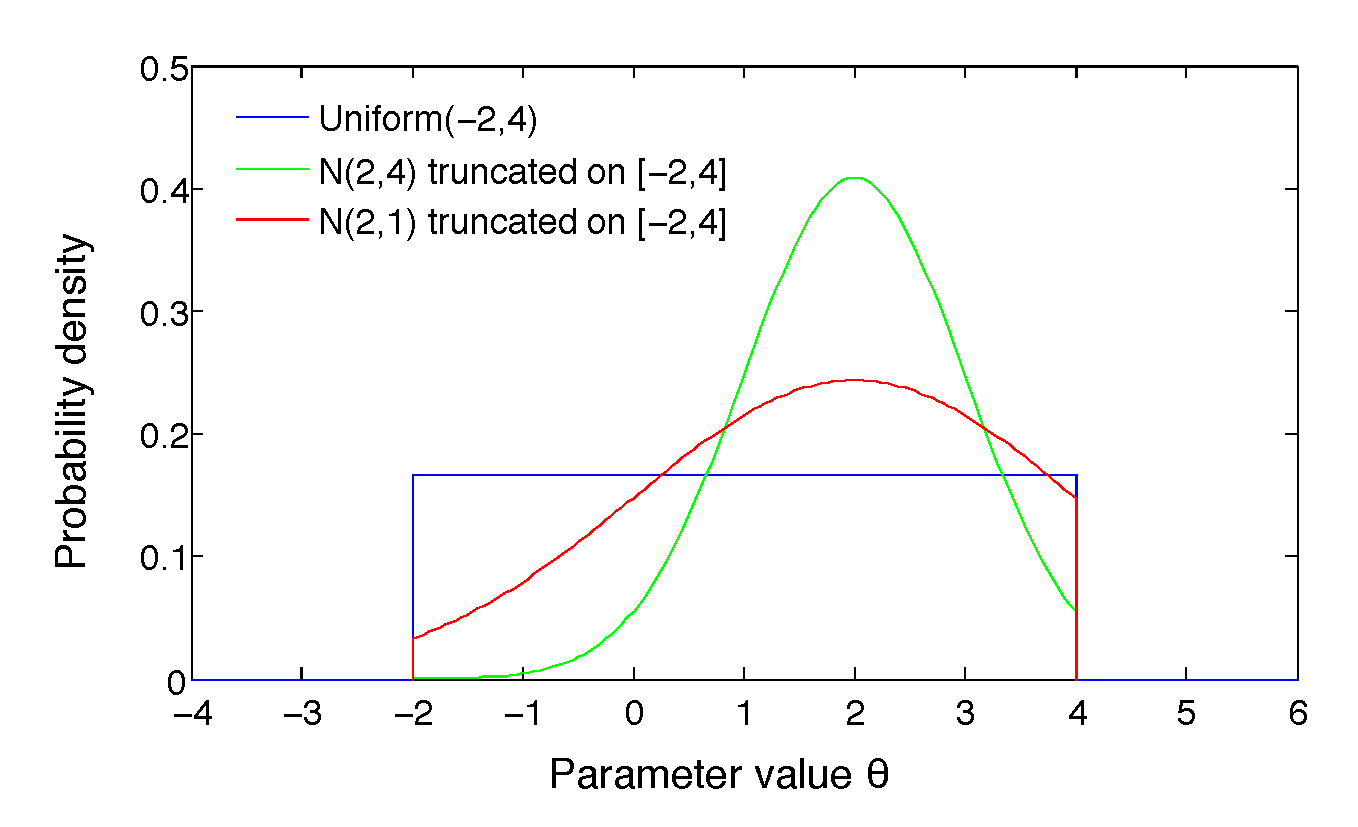
\includegraphics[scale=0.4]{imgs/uniformn.pdf}
\caption{Probability density functions $P(\theta)$ over the interval $[-2,4]$ using an uniform distribution, a truncated normal distribution $\mathcal{N}(2,4)$ and a truncated normal distribution $\mathcal{N}(2,1)$.} 
\label{fig:uniformn}
\end{figure}

\subsection{Instantiation in the dialogue state}
\label{sec:rule-params-instantiation}

Parameters are instantiated in the dialogue state by creating a distinct chance node for each parameter distribution and adding them as parents of their corresponding rule node.  

A parametrised probability rule $r$ with $n$ conditions is thus associated with $n$ parameter nodes $\boldsymbol\theta_{r(1)}, ... \boldsymbol\theta_{r(n)}$.  The probability distribution $P(\boldsymbol\theta_{r(i)})$ is defined as a Dirichlet distribution of dimension $m_i$, where $m_i$ is the number of effects associated with the condition $c_i$ (including the empty effect). Figure \ref{fig:ruleinstantiation_params} illustrates this instantiation procedure with two probability rules.  

The conditional probability distribution of a rule node $r$ given its input variables $I_1,...I_k$ and parameters $\boldsymbol\theta_{r(1)}, ... \boldsymbol\theta_{r(n)}$ is a straightforward adaptation of Equation \eqref{eq:ruledistrib}:
\begin{align}
& P(r\!=\!e \, | \, I_1\!=\!i_1,... I_k\!=\!i_k \, ; \, \boldsymbol\theta_{r(1)}, ... \boldsymbol\theta_{r(n)})  = P(E_i = e \, ; \, \boldsymbol\theta_{r(i)}) \\
& \; \; \; \; \; \; \; \; \text{ where } i = \min_i (c_i \text{ is satisfied with } I_1\!=\!i_1 \land ... I_k\!=\!i_k) \nonumber
\end{align}

The parameters of utility rules are instantiated in a similar manner, as shown in Figure \ref{fig:ruleinstantiation_params2}. The corresponding utility distribution is adapted from Equation \ref{eq:utildistrib} as follows:
\begin{align}
& U_r(I_1\!=\!i_1,... I_k\!=\!i_k, A_1\!=\!a_1,... A_l\!=\!a_l \, ; \, \boldsymbol\theta_{r(1)} ... \boldsymbol\theta_{r(n)}) \nonumber \\
& = U_i(A_1\!=\!a_1,... A_l\!=\!a_l \, ; \, \boldsymbol\theta_{r(1)} ... \boldsymbol\theta_{r(n)})  \label{eq:utildistrib}\\
&  \; \; \; \; \; \; \; \;  \; \; \; \text{ where } i = \min_i (c_i \text{ is satisfied with } I_1 \land ... I_k) \nonumber
\end{align}

\begin{figure}[h!]
\centering
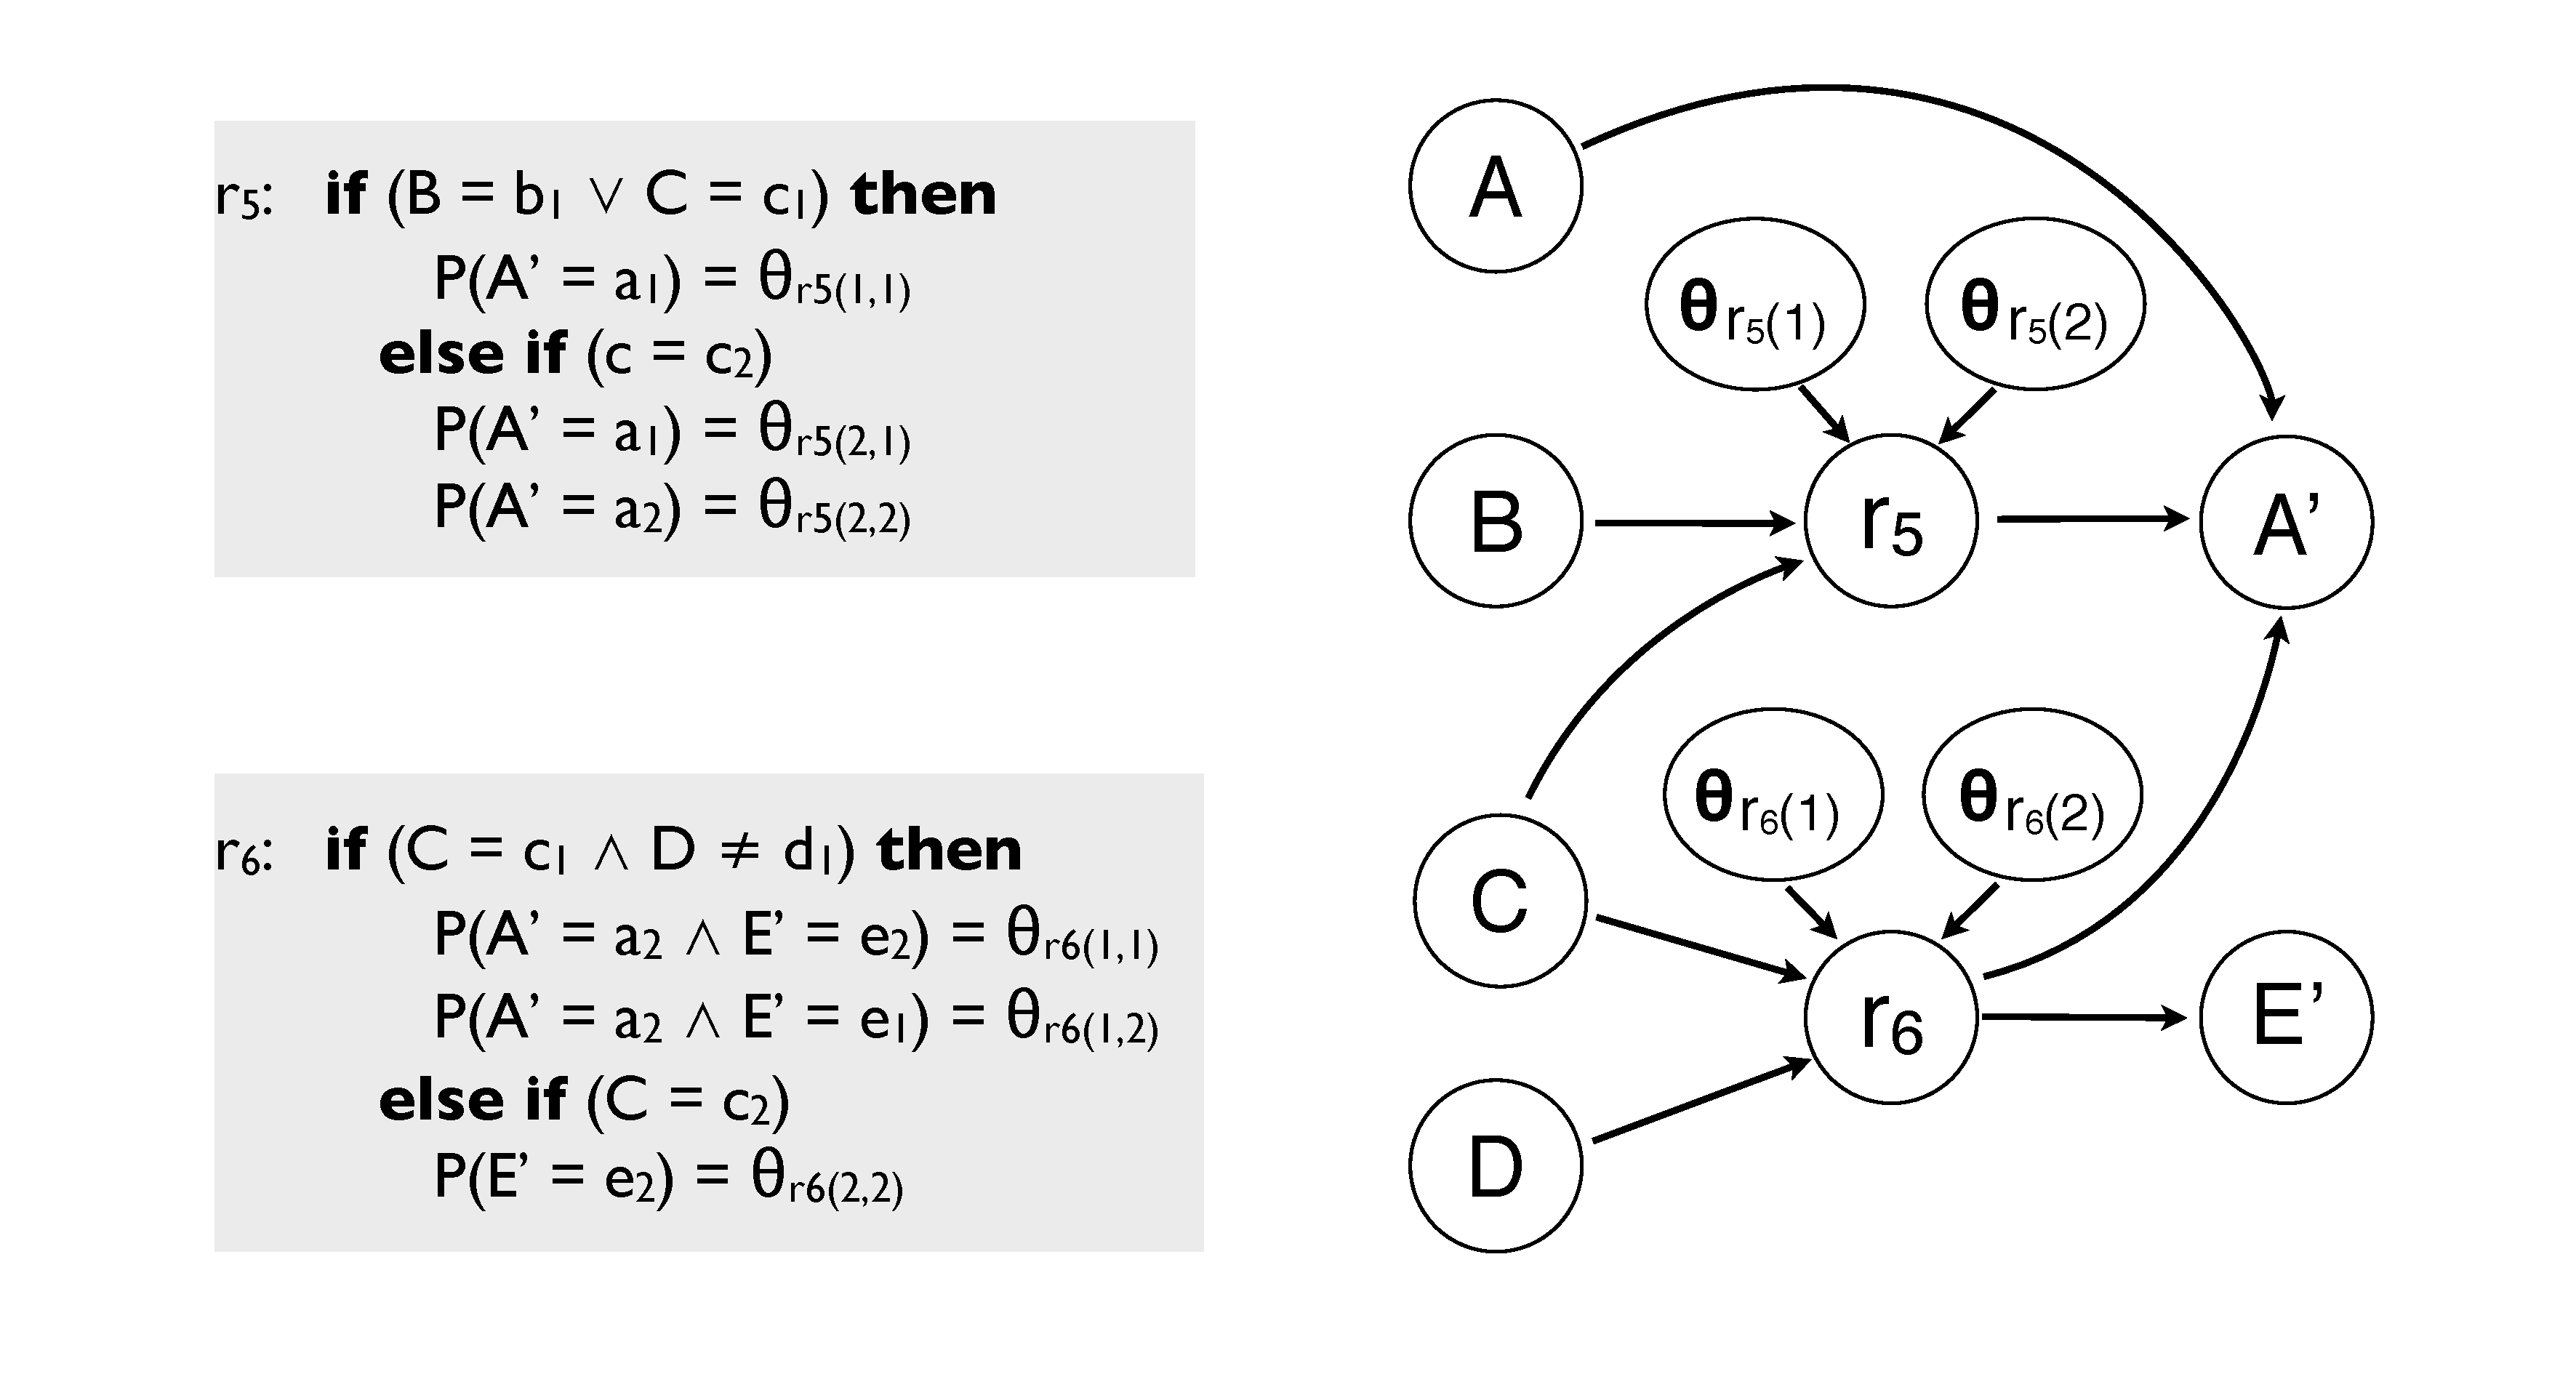
\includegraphics[scale=0.25]{imgs/ruleinstantiation_params.pdf}
\caption{Example of instantiation for two parametrised probability rules $r_5$ and $r_6$.}
\label{fig:ruleinstantiation_params}
\end{figure}


\begin{figure}[h!]
\centering
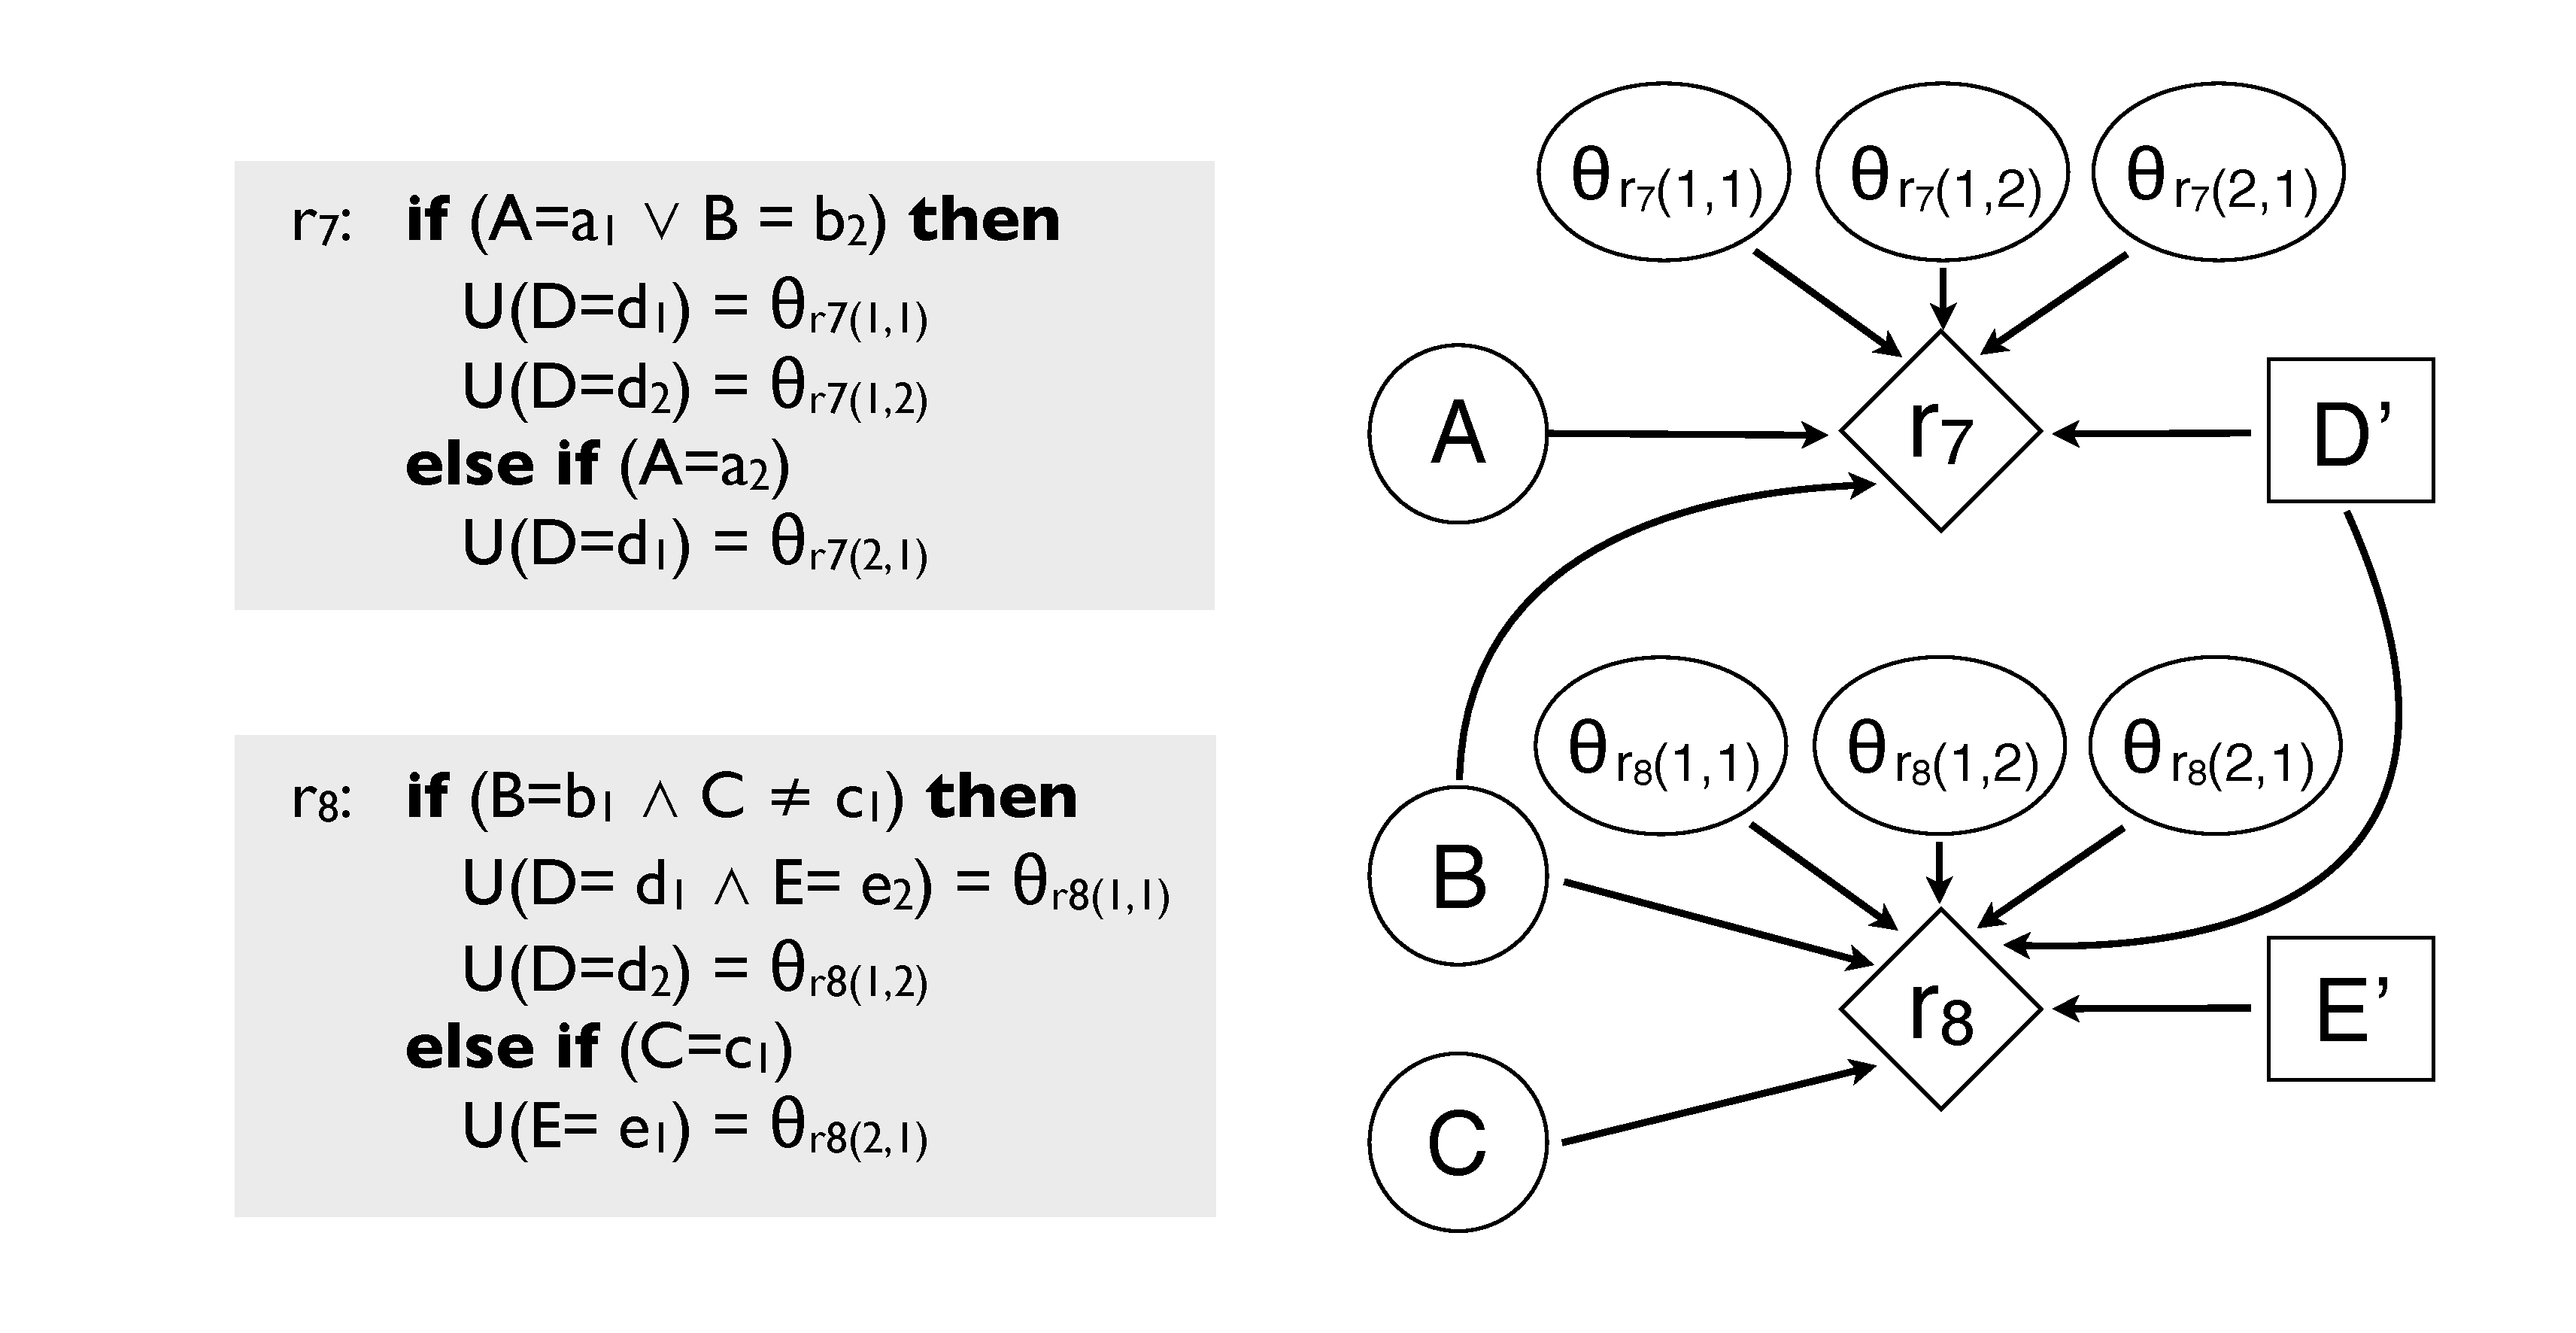
\includegraphics[scale=0.25]{imgs/ruleinstantiation2_params.pdf}
\caption{Example of instantiation for two parametrised utility rules $r_7$ and $r_8$.}
\label{fig:ruleinstantiation_params2}
\end{figure}


\section{Supervised learning of rule parameters}
\label{sec:rule-supervised}

Once the rule parameters are instantiated as nodes in the dialogue state, one can calculate their posterior distribution $P(\boldsymbol\theta \, | \, \mathcal{D})$ after observing a particular data set $\mathcal{D}$ using standard algorithms for probabilistic inference. The estimation of rule parameters corresponds to a learning problem with partial data (cf. Section \ref{sec:learning}), since many chance variables (e.g. rule nodes) are not directly observed. The posterior distribution $P(\boldsymbol\theta \, | \, \mathcal{D})$ is thus no longer guaranteed to remain in the same distribution family as their prior distributions.  The solution adopted in this thesis is to approximate the parameter distributions via sampling techniques, as shall be explained below. 

This chapter focuses on the estimation of rule parameters from Wizard-of-Oz data.  In such setting, parameter estimation is achieved by cycling through the data sample one after the other and gradually refining the parameter distributions based on them. We describe in the next pages the generic representation of the training data as well as the learning algorithm that uses them. 

\subsection{Wizard-of-Oz training data}
\label{sec:rule-supervised-oz}

Wizard-of-Oz data are recorded interactions between human users and a dialogue system that is remotely controlled by a human expert ``behind the curtains''. These recorded interactions can be represented and annotated in multiple ways.  For the particular purpose of estimating the parameters of dialogue management models, we can extract a sequence of state-action pairs $\mathcal{D} = \{\langle \mathcal{B}_i, a_i \rangle : 1 \leq i \leq n\}$, where $\mathcal{B}_i$ corresponds to the dialogue state at time $i$, and $a_i$ is the associated action performed by the wizard.  The number $n$ corresponds to the total number of actions selected by the wizard in the collected interactions. 

The aim of the dialogue state $\mathcal{B}_i$ is to represent the current conversational situation at time $i$ as it was perceived by the wizard.  Its representation is therefore domain-specific, but usually encodes at least the last system action and the last user dialogue act as well as important contextual features.  The dialogue state is encoded as a Bayesian network to reflect state uncertainty (in the form of e.g. uncertain hypotheses generated by the ASR/NLU components) and dependences amongst state variables. Associated to each dialogue state is the corresponding action selected by the wizard at that state. This action can of course be void if the wizard decides to take no action at that specific step in the dialogue. The sequence of state-action pairs $\mathcal{D}$ was in our work automatically extracted from the collected interactions, without any manual annotation.  

In order to perform parameter estimation on Wizard-of-Oz data, a key element is the assumption that the wizard is a rational agent and will tend to select actions that are deemed most useful in their respective dialogue state. It should be stressed that the agent is only assumed to act rationally \textit{given} the perceived (uncertain) dialogue state. The wizard must indeed act on the basis of the same ``noisy'' inputs (with e.g. speech recognition errors) as a real dialogue system would do.  As a consequence, the wizard may behave incorrectly if the provided inputs contain erroneous hypotheses. Hence, the assumption of rationality does not equate to an assumption of omniscience on the part of the wizard. 

Practically, this assumption implies that the likelihood $P_{\mathcal{B}_i}(a_i \, ; \, \boldsymbol\theta)$ of a wizard action $a_i$ in a particular dialogue state $\mathcal{B}_i$ with parameters $\boldsymbol\theta$ will be assigned a high probability if the utility of the action $a_i$ is high relative to other actions, and a low probability otherwise.  

It should be noted that many conversational situations allow for multiple, equally ``correct'' system responses.  This characteristic of verbal interactions transpires in the state-action pairs of Wizard-of-Oz data sets, as one can occasionally observe similar dialogue states being assigned to distinct wizard actions. The wizard actions should therefore be viewed as an indication of good conversational behaviour, but do not constitute absolute gold standards in the traditional NLP sense of being the uniquely appropriate output for the given dialogue state. The existence of multiple potential responses also entails that the accuracy of the learned decision models remains contingent on the degree of internal consistency of the wizard actions. 

\subsection{Learning cycle}
\label{sec:rule-supervised-learning}

The goal of the learning process is to estimate the posterior distribution $P(\boldsymbol\theta \, | \, \mathcal{D})$ over the rule parameters given the collected Wizard-of-Oz data set. The procedure operates in an incremental fashion by traversing the (state,action) pairs one by one and re-estimating the posterior distribution after each pair.  

\subsubsection*{Likelihood distribution}

The most important element of the learning cycle is the definition of the distribution $P_{\mathcal{B}_i}(a_i \, ; \, \boldsymbol\theta)$, which specifies the likelihood of the wizard action $a_i$ in a dialogue state $\mathcal{B}_i$ with parameters $\boldsymbol\theta$. The purpose of this likelihood is intuitively to favour the parameter values that provide a good fit for the wizard action choices. This is practically achieved by defining the likelihood as the relative utility of the action $a_i$ compared to all other actions: 
\begin{equation}
P_{\mathcal{B}_i}(a_i \, ; \, \boldsymbol\theta) \leftarrow \dfrac{U_{\mathcal{B}_i}(a_i \, ; \, \boldsymbol\theta) - U_{\mathrm{min}}}{\sum_{a \in Val(A)} (U_{\mathcal{B}_i}(a  \, ; \, \boldsymbol\theta) - U_{\mathrm{min}})} \label{eq:likelihood}
\end{equation}

Optimal parameter values will therefore assign a high utility to the action $a_i$ and low utilities to the other actions. Note that Equation \eqref{eq:likelihood} includes a minimal utility threshold $U_{\mathrm{min}}$, which is used to ensure that the likelihood remains positive. This threshold can be provided by the system designer or automatically derived from the domain models. 

\subsubsection*{Posterior parameter distribution}

Given the aforementioned likelihood distribution, the posterior distribution over the parameters is defined via Bayes' rule: 
\begin{equation}
P_{\mathcal{B}_i}(\boldsymbol\theta \, | \, a_i) = \eta P_{\mathcal{B}_i}(a_i \, ; \, \boldsymbol\theta) \ P(\boldsymbol\theta )
\end{equation}

The factor $\eta$ is used for normalisation. It should be noted that the value range for most parameters is typically continuous, and includes as a consequence an infinite number of possible values. Inference in hybrid graphical models including both continuous and discrete variables is known to be a difficult problem.  Two types of solutions can be distinguished:
\begin{itemize}
\item The first solution is to discretise the range of parameter values into distinct buckets, and thereby transform continuous variables into discrete variables, with a number of values equivalent to the number of buckets employed for the discretisation.
\item The second solution is to retain the continuous nature of the parameters, but simplify the inference through the use of sampling techniques.  
\end{itemize}

Although both solutions are implemented in the \opendial toolkit, sampling techniques such as likelihood weighting have proved to be in practice more efficient and scalable than discretisation. 

After sampling, the full joint distribution $P_{\mathcal{B}_i}(\boldsymbol\theta \, | \, a_i)$ is factored into its individual parameter variables. This factoring is a simplifying assumption, since parameter independence is theoretically no longer guaranteed when handling partially observed data. 
%:\begin{equation}
%P_{\mathcal{B}_i}(\boldsymbol\theta | a_i) = \prod_{\theta_j \in \boldsymbol\theta} P_{\mathcal{B}_i}(\theta_j | a_i)
%\end{equation}

\subsubsection*{Maintenance of the posterior}

The posterior distributions on the parameter values described above take the form of a collection of sampled values. These sampled values can theoretically be exploited to derive corresponding parametric distributions such as Gaussian and Dirichlet distributions.  This derivation is however problematic for a number of reasons.  First, the determination of the distribution family that underlie the sampled values is not straightforward, since posterior parameter distributions are no longer guaranteed to remain in the same family as the prior in the case of learning from partial data. Second, the derivation of Dirichlet distribution from samples is a complex process with no closed form solution.\footnote{Some iterative methods for Dirichlet estimation have however been developed, based on e.g. fixed-point and Newton-Raphson iterative schemes \citep{minka2003}.} 

We have consequently adopted a non-parametric representation of the posterior parameter distributions, based on \textit{Kernel Density Estimation} (KDE).  Assume we want to estimate the probability density function $P(X)$ of a continuous variable $X$ based on a set of samples $x_1, ... x_n$.  The kernel density estimator for the variable density is:
\begin{equation}
\hat{P}(X=x) = \frac{1}{nh} \sum_{i=1}^n K\Big(\frac{x-x_i}{h}\Big) \label{eq:kde}
\end{equation}
where $K(\cdot)$ is a \textit{kernel function} and $h$ is a smoothing parameter called the \textit{bandwidth}. Multiple kernel functions can be used, but a common choice is to adopt a Gaussian kernel. The kernel density estimator corresponds in this case to a combination of $n$ Gaussians, each centered on a sample point $x_i$.  This combination of Gaussians is subsequently smoothed according to the bandwidth parameter. Figure \ref{fig:kde} shows an example of kernel density estimator for a continuous variable. Kernel density estimators do not necessitate any particular assumption about the shape of the underlying density function, and are therefore well-suited to represent distributions for which the exact class of distribution is unknown (as in our case).  As we can observe from the figure, they can also capture distributions containing multiple modes. 

\begin{figure}[h]
\centering
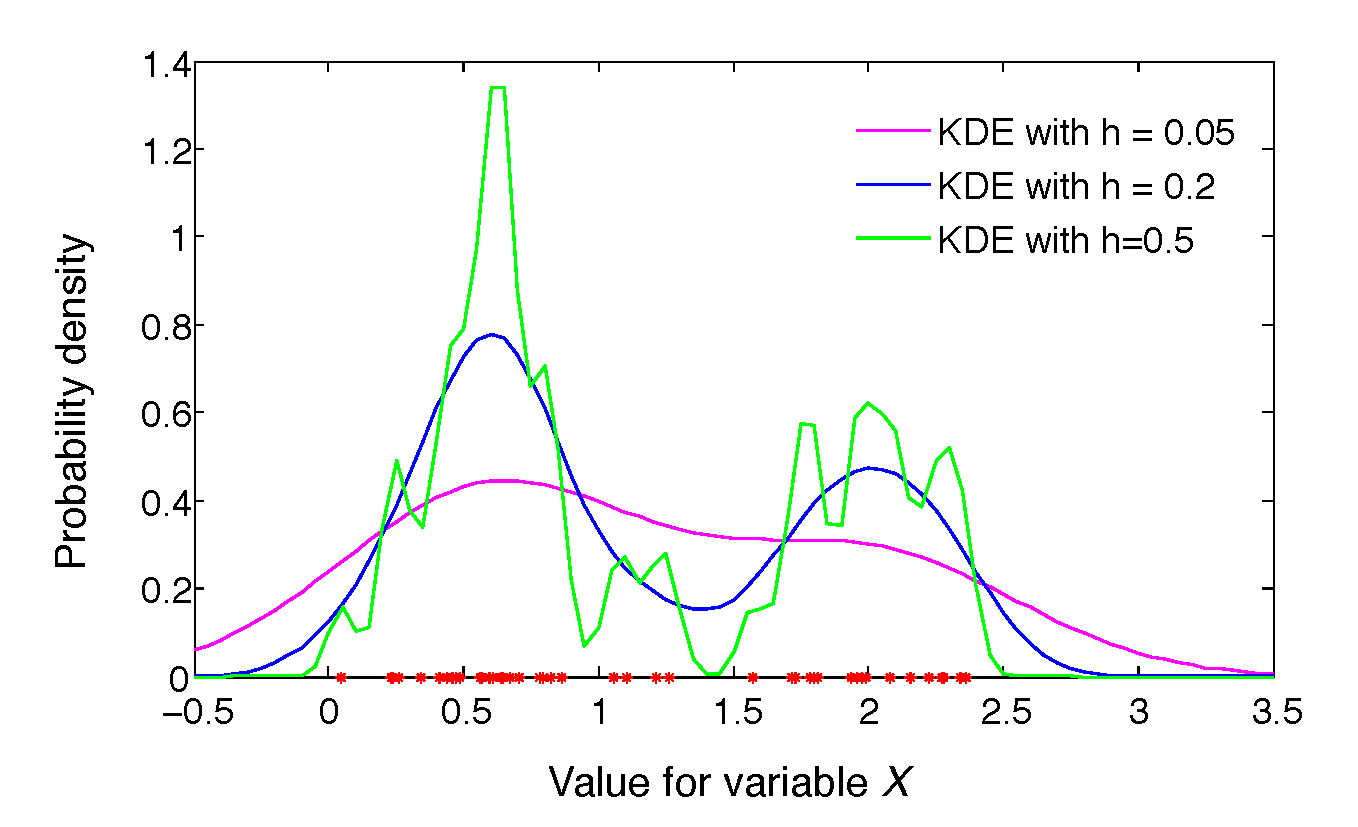
\includegraphics[scale=0.4]{imgs/kde.pdf} 
\caption{Example of kernel density estimator for a continuous variable $X$, based on 50 samples (shown on the X axis).}
\label{fig:kde}
\end{figure}

Univariate parameter distributions (for utility values) are directly represented using Equation \eqref{eq:kde}, while multivariate distributions (arising from Dirichlet priors over probability values) are encoded with a multivariate extension of KDE based on product kernels \citep{Silverman1986}.  Both cases employ Gaussian kernels with a manually tuned bandwidth. 


\subsubsection*{Learning algorithm}

Algorithm \ref{algo:wozlearning} presents the general procedure for estimating model parameters from Wizard-of-Oz data.  The algorithm loops on each instance pair in the training data.  For each pair, the algorithm starts by including the parameters in the input dialogue state for the 
instance and trigger the domain models (line 2 and 3). Given the definition of the wizard action likelihood, the posterior parameter distribution can be estimated via sampling (line 5 and 6).  The posterior distribution for each parameter variable is finally expressed as a kernel density estimator on the value assigned for the parameter in each sample (line 7-9). 

\begin{algorithm}[h!]
\caption{: \textsc{WoZ-learning} ($\mathcal{M}, \boldsymbol\theta, \mathcal{D}, N$)}
\begin{algorithmic}[1] \vspace{1mm}
\REQUIRE $\mathcal{M}$: Rule-structured models for the domain
\REQUIRE $\boldsymbol\theta$: Parameter associated with the models with prior distribution $P(\boldsymbol\theta)$
\REQUIRE $\mathcal{D}$: Wizard-of-Oz data set $\{\langle \mathcal{B}_i, a_i \rangle : 1 \leq i  \leq n\}$
\REQUIRE $N$: Number of samples to draw for each learning example
\ENSURE Posterior distribution $P(\boldsymbol\theta \; | \; \mathcal{D})$ for the parameters  \vspace{1mm}
\FORALL {$\langle \mathcal{B}_i, a_i \rangle \in \mathcal{D}$}
\STATE Set $\mathcal{B}_i \leftarrow \mathcal{B}_i \cup \boldsymbol\theta$
\STATE $\mathcal{B}_i, \mathbf{e} \leftarrow$ \textsc{TriggerModels} ($\mathcal{B}_i, \emptyset,  \mathcal{B}_i$) 
\STATE Let $U_{\mathrm{min}}$ be the minimal threshold for the utilities in $\mathcal{B}_i$ \vspace{2mm} 
\STATE Define likelihood  $P_{\mathcal{B}_i}(a_i \, ; \, \boldsymbol\theta) \leftarrow \dfrac{U_{\mathcal{B}_i}(a_i \, ; \, \boldsymbol\theta) - U_{\mathrm{min}}}{\sum_{a \in Val(A)} (U_{\mathcal{B}_i}(a  \, ; \, \boldsymbol\theta) - U_{\mathrm{min}})} $ \vspace{2mm} 
\STATE Draw $N$ samples $\mathbf{x}_1,...\mathbf{x}_N$ from posterior $P_{\mathcal{B}_i}(\boldsymbol\theta | a_i) = \eta P_{\mathcal{B}_i}(a_i \, ; \, \boldsymbol\theta) \ P(\boldsymbol\theta )$
\FORALL {parameter variable $\theta_j \in \boldsymbol\theta$}
\STATE Set $P(\theta_j) \leftarrow \mathrm{KDE}(\mathbf{x}_1(\theta_j),...\mathbf{x}_N(\theta_j))$
\ENDFOR
\ENDFOR
\RETURN $P(\boldsymbol\theta)$
\end{algorithmic}
\label{algo:wozlearning}
\end{algorithm}


\section{Experiments}
\label{sec:wozlearning-experiments}

We evaluated the learning approach outlined in this chapter in the context of a dialogue policy learning task for a human-robot interaction scenario.  The goal of the experiment, originally presented in \cite{rulebasedmodels-sigdial2012}, was to estimate a the parameters of a rule-structured utility model based on small amount of Wizard-of-Oz data and evaluate its learning performance.  The learning performance was measured in this experiment as the proportion of actions corresponding to the wizard selections. The performance was compared to two baselines where the utility model was represented using classical representations (respectively utility tables and linear functions). We could then show that the model encoded with utility rules was able to reproduce the wizard policy much faster than the more weakly structured baseline representations. 

It should be stressed that the purpose of the experiment is limited to the evaluation of the \textit{learning} performance of the model. The evaluation of the learned model in terms of e.g. qualitative and quantitative metrics of interaction success (and user satisfaction) forms a separate question, which will be addressed in Chapter \ref{chap:user-evaluation}. 

We first describe the dialogue domain used for the experiment, after which we detail the data collection procedure and experimental setup, and finally present and analyse the empirical results. 

\subsection{Dialogue domain}
\label{sec:wozlearning-experiments-domain}

The scenario for the Wizard-of-Oz experiment involved a human user and a Nao robot (nicknamed ``Lenny''), which is a programmable humanoid robot developed by Aldebaran Robotics. Figure \ref{fig:nao} shows a human user interacting with the robot during a data collection experiment. 

\begin{figure}[h]
\begin{center}
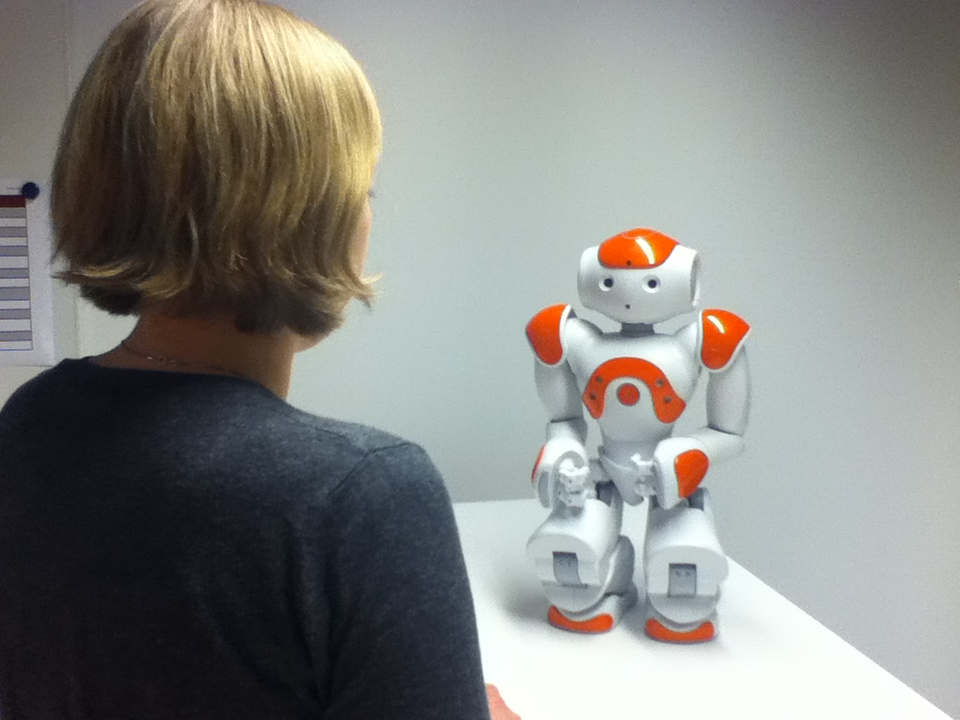
\includegraphics[scale=0.25]{imgs/bilde.jpg}
\end{center}
\caption{Human user interacting with the Nao robot during the Wizard-of-Oz data collection.}
\label{fig:nao}
\end{figure}

The users were instructed to teach the robot a sequence of basic movements such as lifting arms, stepping forward, backward, kneeling down, etc.  The movements could be performed either in consecutive order or in parallel (provided the movements were not in conflict).  The users were free to decide on the movements to perform, and communicated their intention using spoken commands (no gesture recognition was here involved).  The robot was programmed to memorise the instructed sequence and could ``replay'' it at any time.

The list of possible dialogue acts for the user is shown in Table \ref{table:userdas}, and includes a total of 41 dialogue acts (when counting all possible predicate instantiations), amongst which 33 dialogue acts expressing the robot movement to execute, and 8 other dialogue acts expressing feedbacks, acknowledgements, corrections, and generic conversational actions.  To respond to these user inputs, the robot/wizard had at its disposal a repository of 41 possible actions, including both physical and verbal actions such as asking for repetition, clarification or confirmation, and acknowledging the user inputs.  The list of system actions used for the data collection is given in Table \ref{table:systemdas}. 

\renewcommand{\arraystretch}{1.1}

\begin{table}[h]
\begin{minipage}[b]{80mm}
\begin{footnotesize}
\begin{tabular}{p{60mm}} \hdashline \vspace{-2.5mm} 
$\mathrm{MoveArm}(x,y) $ \\ $ \ \ \ \ \ \text{ where } x=\{\mathrm{Left,Right,Both}\} $ \\ $ \ \ \ \ \  \text{ and } y = \{\mathrm{Up,Down,Lateral,}$ \\ $\ \ \ \ \ \ \ \ \ \  \ \ \ \ \ \ \ \ \ \ \ \ \mathrm{Forward,Folded}\}$ \\[0.5mm] \hdashline \vspace{-2.5mm} 
$\mathrm{MoveHead}(y) $ \\ $\ \ \ \ \  \text{ where } y = \{\mathrm{Up,Left,Down,Right}\}$ \\[0.5mm] \hdashline \vspace{-2.5mm} 
$\mathrm{Kneel}$ \\[0.5mm] \hdashline \vspace{-2.5mm}  
$\mathrm{StandUp}$ \\[0.5mm] \hdashline \vspace{-2.5mm} 
$\mathrm{SitDown}$ \\[0.5mm] \hdashline \vspace{-2.5mm} 
$\mathrm{MoveFoot}(x,y) $ \\ $\ \ \ \ \  \text{ where } x = \{\mathrm{Left,Right}\} $ \\ $\ \ \ \ \ \text{ and } y = \{\mathrm{Forward,Backward}\}$ \\[0.5mm] \hdashline \vspace{-2.5mm} 
$\mathrm{Turn}(y) $ \\ $\ \ \ \ \ \text{ where } y = \{\mathrm{Left,Right}\}$  \\[0.5mm] \hdashline \vspace{-2.5mm} 
$\mathrm{Confirm}$ \\[0.5mm] \hdashline \vspace{-2.5mm} 
$\mathrm{Disconfirm}$ \\[0.5mm] \hdashline \vspace{-2.5mm} 
$\mathrm{DoMovements}(y) $ \\ $ \ \ \ \ \  \text{ where } y = \{\mathrm{InParallel,InSequence}\}$\\[0.5mm] \hdashline \vspace{-2.5mm} 
$\mathrm{RepeatAll}$ \\[0.5mm] \hdashline \vspace{-2.5mm} 
$\mathrm{ForgetAll}$ \\[0.5mm] \hdashline \vspace{-2.5mm} 
$\mathrm{Compliment}$ \\[0.5mm] \hdashline \vspace{-2.5mm} 
$\mathrm{SayHello}$ \\[0.5mm] \hdashline \vspace{-2.5mm} 
$\mathrm{SayGoodbye}$ \\[0.5mm] \hdashline \vspace{-2.5mm} 
$\mathrm{SayThankYou}$ \\[0.5mm] \hdashline \vspace{-2.5mm} 
$\mathrm{GoToInitPose}$ \\[0.5mm] \hdashline \vspace{-2.5mm} 
$\mathrm{FollowMe}$ \\[0.5mm] \hdashline \vspace{-2.5mm} 
$\mathrm{Stop}$ \\[0.5mm] \hdashline  
\end{tabular}
\end{footnotesize}
    \caption{List of user actions $a_u$} 
\label{table:userdas}
\end{minipage}
\begin{minipage}[b]{80mm}
\begin{footnotesize}
\begin{tabular}{p{60mm}} \hdashline \vspace{-2.5mm} 
$\mathrm{Demonstrate}(z)$ \\ $\ \ \ \ \ \text { where } z = \{\mathrm{MoveArm}(x,y), $ \\ $\ \ \ \ \ \ \ \ \ \ \ \ \ \ \ \ \ \ \ \ \ \ \ \ \  \mathrm{MoveHead}(y),\mathrm{Kneel}, $ \\ $\ \ \ \ \ \ \ \ \ \ \ \ \ \ \ \ \ \ \ \ \ \ \ \ \  \mathrm{StandUp},\mathrm{SitDown}, $ \\ $\ \ \ \ \ \ \ \ \ \ \ \ \ \ \ \ \ \ \ \ \ \ \ \ \  \mathrm{MoveFoot}(x,y), \mathrm{Turn}(y)\}$ \\ $\ \ \ \ \ \text{ and } x, y \text{ take the same values}$ \\ $\ \ \ \ \ \ \ \ \ \ \ \ \ \ \ \ \ \ \ \ \text{as for the user actions}$ \\[0.5mm] \hdashline \vspace{-2.5mm} 
$\mathrm{AskConfirmation}$ \\[0.5mm] \hdashline \vspace{-2.5mm} 
$\mathrm{RegisterMove}$ \\[0.5mm] \hdashline \vspace{-2.5mm} 
$\mathrm{UndoMove}$ \\[0.5mm] \hdashline \vspace{-2.5mm} 
$\mathrm{AskRepeat}$ \\[0.5mm] \hdashline \vspace{-2.5mm} 
$\mathrm{Acknowledgement}$ \\[0.5mm] \hdashline \vspace{-2.5mm} 
$\mathrm{AskIntention}$ \\[0.5mm] \hdashline \vspace{-2.5mm} 
$\mathrm{DemonstrateAll}$ \\[0.5mm] \hdashline \vspace{-2.5mm} 
$\mathrm{ForgetAll}$ \\[0.5mm] \hdashline \vspace{-2.5mm} 
$\mathrm{StopMove}$ \\[0.5mm] \hdashline \vspace{-2.5mm} 
$\mathrm{FollowUser}$ \\[0.5mm] \hdashline \vspace{-2.5mm} 
$\mathrm{SayThankYou}$ \\[0.5mm] \hdashline \vspace{-2.5mm} 
$\mathrm{SayHello}$ \\[0.5mm] \hdashline \vspace{-2.5mm} 
$\mathrm{SayGoodbye}$  \\[0.5mm] \hdashline 
\end{tabular}
\end{footnotesize}
\caption{List of system actions $a_m$} 
\label{table:systemdas}
\end{minipage}
\end{table}

\subsection{Wizard-of-Oz data collection}
\label{sec:wozlearning-experiments-woz}

The Wizard-of-Oz data set consist of a set of recorded dialogues, where each dialogue involved a single human subject and the Nao robot.  The dialogues are relatively short, with an average duration of about five minutes. The task (described above) was common to all dialogues.


At the system level, the robot was equipped with multiple modules to control both the verbal and physical behaviour of the robot \begin{itemize}
\item On the understanding side, the speech stream was recorded by four microphones placed on the robot head and passed to an off-the-shelf speech recogniser (Vocon 3200 from Nuance).  The speech recogniser used a small hand-crafted recognition grammar as language model, and the corresponding user dialogue acts were derived from the ASR hypotheses by a template-based recognition model. 
\item On the generation side, a shallow generation model was in charge of the surface realisation of the verbal actions.  The surface string was synthesised via an off-the-shelf TTS module embarked on the robot.
\item The execution the physical actions selected by the wizard was delegated to a separate module, responsible for  planning the robot movements and controlling its motors in real-time, based on the libraries available on the robot platform. 
\end{itemize}

All components are connected to the shared belief state, and read/write to it as they process their data flow.  Figure \ref{fig:exp1_architecture} illustrates the general system architecture and its connection with the robotic platform. The dialogue management module is naturally replaced by the wizard during data collection. 

\begin{figure}[h]
\begin{center}
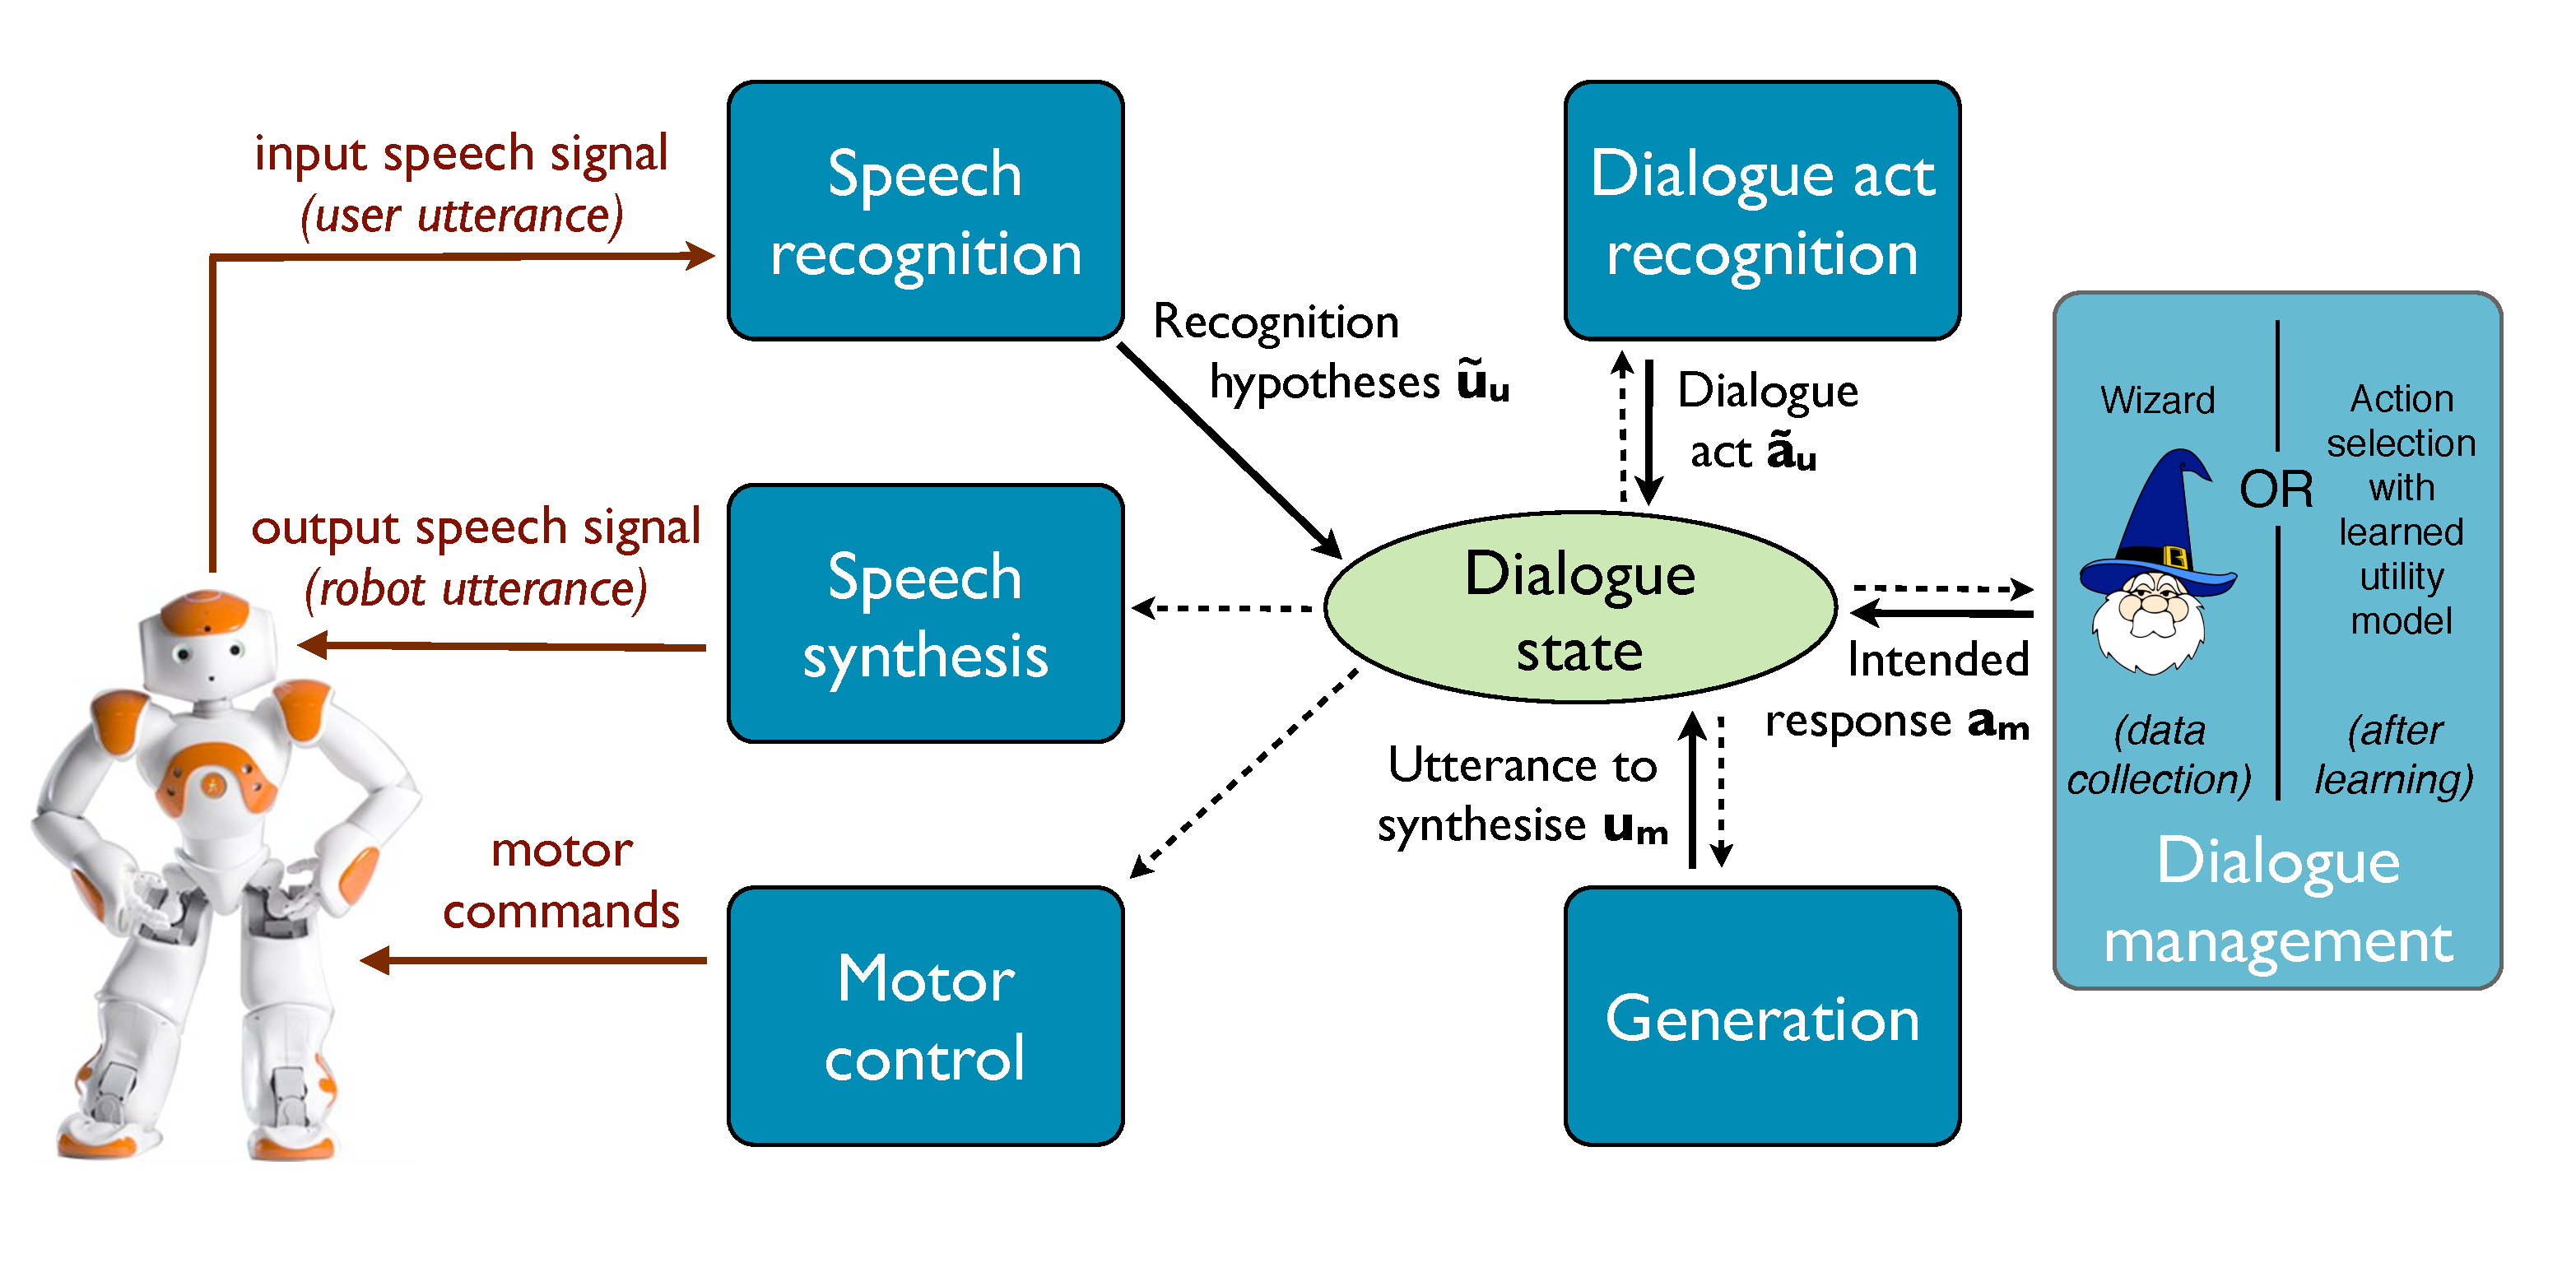
\includegraphics[scale=0.30]{imgs/exp1_architecture.pdf}
\end{center}
\caption{System architecture used for the experiment.}
\label{fig:exp1_architecture}
\end{figure}

We collected a total of 20 interactions with 7 distinct users, for a total of 1020 system turns, summing to around 1h of interaction.  All the interactions were performed in English.  As the speech recogniser relied on a grammar-based language model of limited size, the users were briefed before each experiment about the speech recognition capabilities of the robot in order to adjust their expectations about what the robot could and could not understand. 

The wizard only had access to the N-best list $\tilde{a}_u$ provided by the dialogue action recognition engine, and could select the action to perform from a list of alternatives.  Each selected action $a_m$ was recorded along with the complete dialogue state $\mathcal{B}$ in effect at the time of the selection.

We detail in the two following pages two recorded excerpts of Wizard-of-Oz interactions.  The user utterances are presented as N-best lists of speech recognition hypotheses. 

\begin{Transcript}[p!]
\begin{dialogue} \vspace{3mm}
\speak{Human} $\begin{bmatrix}\text{ hello Lenny} & 0.22 \\
\text{ follow me} & 0.20 \\
\text{ hi Lenny} & 0.53 \end{bmatrix}$ \vspace{3mm}
\speak{Robot} \ \ \ Hello there!\vspace{3mm}
\speak{Human} $\begin{bmatrix}\text{ move your left arm up} & 0.41 \\
\text{ move the left arm up} & 0.27 \\
\text{ put your left arm up} & 0.30 \end{bmatrix}$ \vspace{3mm}
\speak{Robot} \ \ \ Sure! \vspace{2mm}\\
\direct{\refer{Robot} executes the movement $\textrm{Move(LeftArm,Up)}$} \\
\direct{\refer{Robot} waits a few seconds} \vspace{2mm}
\speak{Robot} \ \ \ Was that correct? \vspace{3mm}
\speak{Human} $\begin{bmatrix}\text{ yes} & 0.88 \\
\text{ thanks} & 0.10 \\
\text{ put your left arm up} & 0.30 \end{bmatrix}$ \vspace{2mm} \\
\direct{\refer{Robot} registers the movement as confirmed} \vspace{3mm}
\speak{Robot} \ \ \ Great \vspace{3mm}
\speak{Human} $\begin{bmatrix}\text{ move your right arm up at the same time} & 0.26 \\
\text{ put the right arm up at the same time} & 0.32 \\
\text{  move the right arm up at the same time} & 0.38 \end{bmatrix}$ \vspace{3mm}
\speak{Robot} \ \ \ Let's see \vspace{1mm} \\
\direct{\refer{Robot} executes movement $\textrm{Move(BothArms,Up)}$} \vspace{2mm}
\speak{Robot} \ \ \ Was that correct? \vspace{3mm}
\speak{Human} $\begin{bmatrix}\text{ kneel} & 0.25 \\
\text{ thanks} & 0.14 \\
\text{  no} & 0.57 \end{bmatrix}$  \vspace{2mm} \\
\direct{\refer{Robot} discards last movement and goes back to previous position} \vspace{2mm}
\speak{Robot} \ \ \ What should I do then?  \\
\end{dialogue}
\vspace{-4mm} \hspace{1cm}\direct{...} \vspace{3mm}
\caption{User interaction with wizard-controlled robot, first excerpt}
\end{Transcript}

\begin{Transcript}[p!]
\vspace{4mm} \hspace{1cm} \direct{...}
\begin{dialogue} 
\speak{Human} $\begin{bmatrix}\text{ stop} & 0.25 \\
\text{ stand up} & 0.41 \\
\text{ no} & 0.25 \end{bmatrix}$ \vspace{3mm}
\speak{Robot} Let's see \vspace{1mm} \\
\direct{\refer{Robot} executes movement $\mathrm{StandUp}$} \vspace{3mm}
\speak{Human}  $\begin{bmatrix}\text{ put your right arm forward} & 0.31 \\
\text{ move your right arm forward} & 0.36 \\
\text{ move the right arm forward} & 0.30 \end{bmatrix}$ \vspace{2mm} \\
\direct{\refer{Robot} registers movement $\mathrm{StandUp}$ as implicitly confirmed} \vspace{2mm}
\speak{Robot} Let's see \vspace{1mm} \\
\direct{\refer{Robot} executes movement $\mathrm{Move(RightArm,Forward)}$} \vspace{3mm}
\speak{Human} $\begin{bmatrix}\text{ move forward the left arm} & 0.31 \\
\text{ lower the left arm} & 0.35 \\
\text{ lower both arms} & 0.29 \end{bmatrix}$ \vspace{3mm}
\speak{Robot} Sorry, could you repeat? \vspace{3mm}
\speak{Human} $\begin{bmatrix}\text{ raise your left arm} & 0.28 \\
\text{ lift your right arm} & 0.31 \\
\text{ lift your left arm} & 0.37 \end{bmatrix}$ \vspace{3mm}
\speak{Robot} Sure \vspace{1mm} \\
\direct{\refer{Robot} executes movement $\mathrm{Move(LeftArm,Up)}$} \\
\direct{\refer{Robot} waits a few seconds} \vspace{3mm}
\speak{Robot} Should I do it like this? \\
\speak{Human} $\begin{bmatrix}\text{ kneel} & 0.23 \\
\text{ wrong} & 0.22 \\
\text{ no} & 0.47 \end{bmatrix}$ \vspace{3mm} \\
\direct{\refer{Robot} discards last movement and goes back to previous position} \vspace{2mm}
\speak{Robot} What should I do then?  \vspace{3mm}
\speak{Human} $\begin{bmatrix}\text{ move your left arm up} & 0.29 \\
\text{ move the left arm up} & 0.34 \\
\text{ move the left arm down} & 0.28 \end{bmatrix}$ \vspace{3mm} \\
\end{dialogue}
\vspace{-4mm} \hspace{1cm} \direct{...} \vspace{3mm}
\caption{User interaction with wizard-controlled robot, second excerpt}
\end{Transcript}

\subsection{Experimental setup}
\label{sec:wozlearning-experiments-setup}

The main question we decided to address in this experiment is the following: how much does the rule structure contribute to the parameter estimation of a given probabilistic model, especially for domains with limited amounts of available data?  The objective of the experiment was to learn the rule parameters of a utility model based on training data gathered from Wizard-of-Oz interactions. The parameters correspond here to the utilities of the various system actions depending on the current state.


\subsubsection*{Dialogue state}

The dialogue state designed for the experiment consisted of fives variables: \begin{enumerate}
\item The last user dialogue act $a_u$ (with the values shown in Table \ref{table:userdas})
\item The last system action $a_m$ (with the values shown in Table \ref{table:systemdas})
\item The recorded sequence of movements, encoded as a list (cf. Section \ref{sec:amodelling})
\item The last physical movement demonstrated by the robot
\item Finally, a (regularly updated) variable expressing the number of seconds elapsed since the last user or system action. 
\end{enumerate}

\subsubsection*{Baseline models}

The experiment relied on two baselines that express the utility model of the domain based on traditional representations: \begin{enumerate}
\item The first baseline is a plain utility table that maps every combination of state values and actions to a particular utility.  For a given set of state variables $X_1,...X_n$, 
the utility is therefore defined by: 
\begin{equation}
U(X_1=x_1,...X_n=x_n, a_m) = \theta_{(x_1,...x_n, a_m)}
\end{equation}
where the $\theta$ value corresponds to the utility encoded in the table for the state-action pair. The number of parameters required to determine the utility table is therefore $|Val(X_1)| \times ... |Val(X_n)| \times |Val(a_m)|$. 
\item The second baseline defines the utility of a given action as a linear combination of values -- one for each state variable.  The total utility is thus determined as:
\begin{equation}
U(X_1=x_1,...X_n=x_n, a_m) = \sum_{i=1}^{n} \theta_{(x_i, a_m)}
\end{equation}
where $\theta_{(x_i, a_m)}$ corresponds to the utility weight of the variable value $x_i$ for the action $a_m$.  Note that the weights are specific to a given action value. The number of required parameters is here reduced to $|Val(a_m)| \times (|Val(X_1)| + ... |Val(X_n)|$ compared to the plain utility table.  This baseline hinges however on the assumption that the total utility of a given action can be decomposed as a linear combination of weights associated with each state variable value.
\end{enumerate}

\subsubsection*{Rule-structured model}

The two baselines were compared to a utility model structured with 15 utility rules. The interested reader is invited to browse these rules in Appendix \ref{chap:domainspecs}. The rule structure was designed by hand, while the parameters (in this case, utility values) remained unknown. 

\subsubsection*{Parameter estimation}

Figure \ref{fig:exp1_baselines} offers a graphical comparison of the utility models produced for the two baselines and the rule-structured approach.  The careful reader may notice that the two baselines are essentially ``flattened'' or unstructured versions of the rule-based model.  The input and output variables remain identical in all three models. However, the two baselines directly associate each state-action combination to a utility value, while the rule-structured approach uses rule nodes as intermediaries to define the overall utility.  


\begin{figure}[h]
\centering
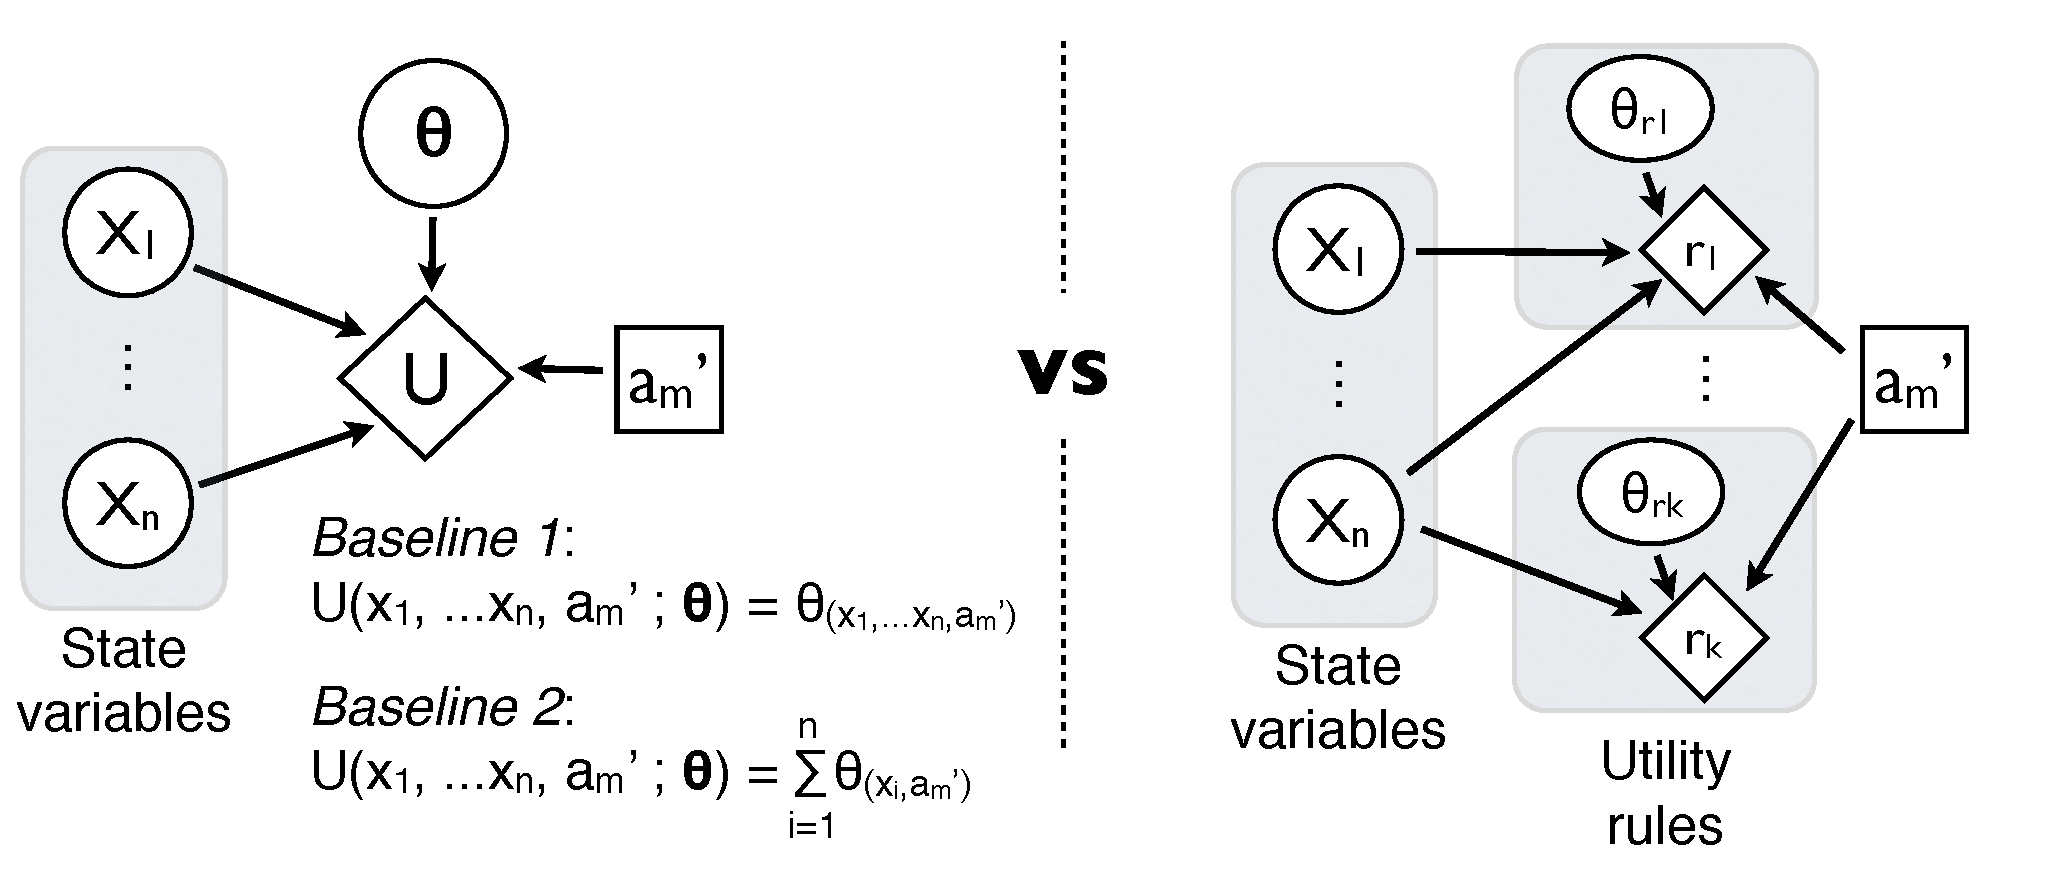
\includegraphics[scale=0.40]{imgs/exp1_baselines.pdf}
\caption{Baseline utility models (left) compared to the rule-structured utility model (right).}
\label{fig:exp1_baselines}
\end{figure}


The parameter estimation procedure was identical for the three models, and followed the Bayesian learning approach detailed in Section \ref{sec:rule-supervised-learning}. For the baseline models, the function \textsc{triggerModels}(...) was replaced by a construction of a single utility node connected to the system action, as illustrated in Figure \ref{fig:exp1_baselines}.  The number of parameters was 8962 for the plain utility table, 581 for the linear model, and 17 for the utility rules.

The parameter distributions for all utilities (both in the baseline and rule-based models) were initialised with uniform priors on the interval $[-1,6]$ and were progressively refined as more data points are processed.  

\subsubsection*{Evaluation metric}

Given the utility models defined above, the action to execute was determined by searching for the action associated with the maximum utility in the current state and selecting it. In this particular experiment, the utility maximisation only considered the current (immediate) utility and did not perform forward planning.

The data collected from the Wizard-of-Oz interactions was split into a training set composed of 765 state-action pairs (75 \% of the gathered data) and a held-out test set with 255 actions (remaining 25 \%). The resulting training set was used to estimate the utility parameters for the three models. The estimated parameters were then applied to compare the \textit{accuracy} of the three models.  The accuracy of a given utility model is here defined as the percentage of actions corresponding to the action selected by the wizard.  The accuracy results of the three models were evaluated at various learning stage to analyse and compare their learning performance. We calculated the accuracy by sampling over the parameters, performing inference over the resulting models, and finally averaging over the inference results.  

\subsection{Empirical results and analysis}
\label{sec:wozlearning-experiments-results}

Table \ref{table} provides the accuracy results for the three utility models -- that is, the plain utility table, the linear model, and the rule-structured model. The differences between the rule-structured model and the baselines are statistically significant using Bonferroni-corrected paired $t$-tests, with $p$-value $< 0.0001$.  The 17\% of actions that remain labelled as incorrect are mainly due to the high degree of noise in the data set, and the sometimes inconsistent behaviour of the wizard (especially regarding the use of e.g. clarification requests). 

\begin{table}[h]
\begin{center}
\begin{tabular}{|l|c|} \hline
\textit{Type of model} & \textit{Accuracy (in \%) } \\ \hline \hline
Plain model & 67.35 \\ \hline
Linear model & 61.85 \\ \hline
Rule-structured model & \textbf{82.82} \\ \hline
\end{tabular}
\end{center}
\vspace{-2mm}
\caption{Accuracy results for the three models on a held-out test after parameter estimation.}
\vspace{-2mm}
\label{table}
\end{table}

The learning curves for the three models are shown in Figure \ref{results}.   Given its considerably smaller number of parameters, the rule-structured model is able to converge to near-optimal values after observing only a small fraction of the training set.  The incorporation of domain knowledge via the rule structure has a clearly beneficial effect on the learning performance and on the generalisation capacity of the model.  As the figure shows, the baseline models do also improve their accuracies over time, but at a much slower rate.   The linear model is comparatively faster than the plain model, but levels off towards the end, possibly due to the non-linearity of some dialogue strategies.  The plain model continues its convergence and would probably reach an accuracy similar to the rule-structured model if given much larger amounts of training data. 

Note that since the parameters are initially uniformly distributed, the accuracy is already non-zero before learning, since a random assignment of parameters has a low but non-zero chance of leading to the right action.


\begin{figure*}[p!]
\begin{center}\subfigure[Linear scale]{
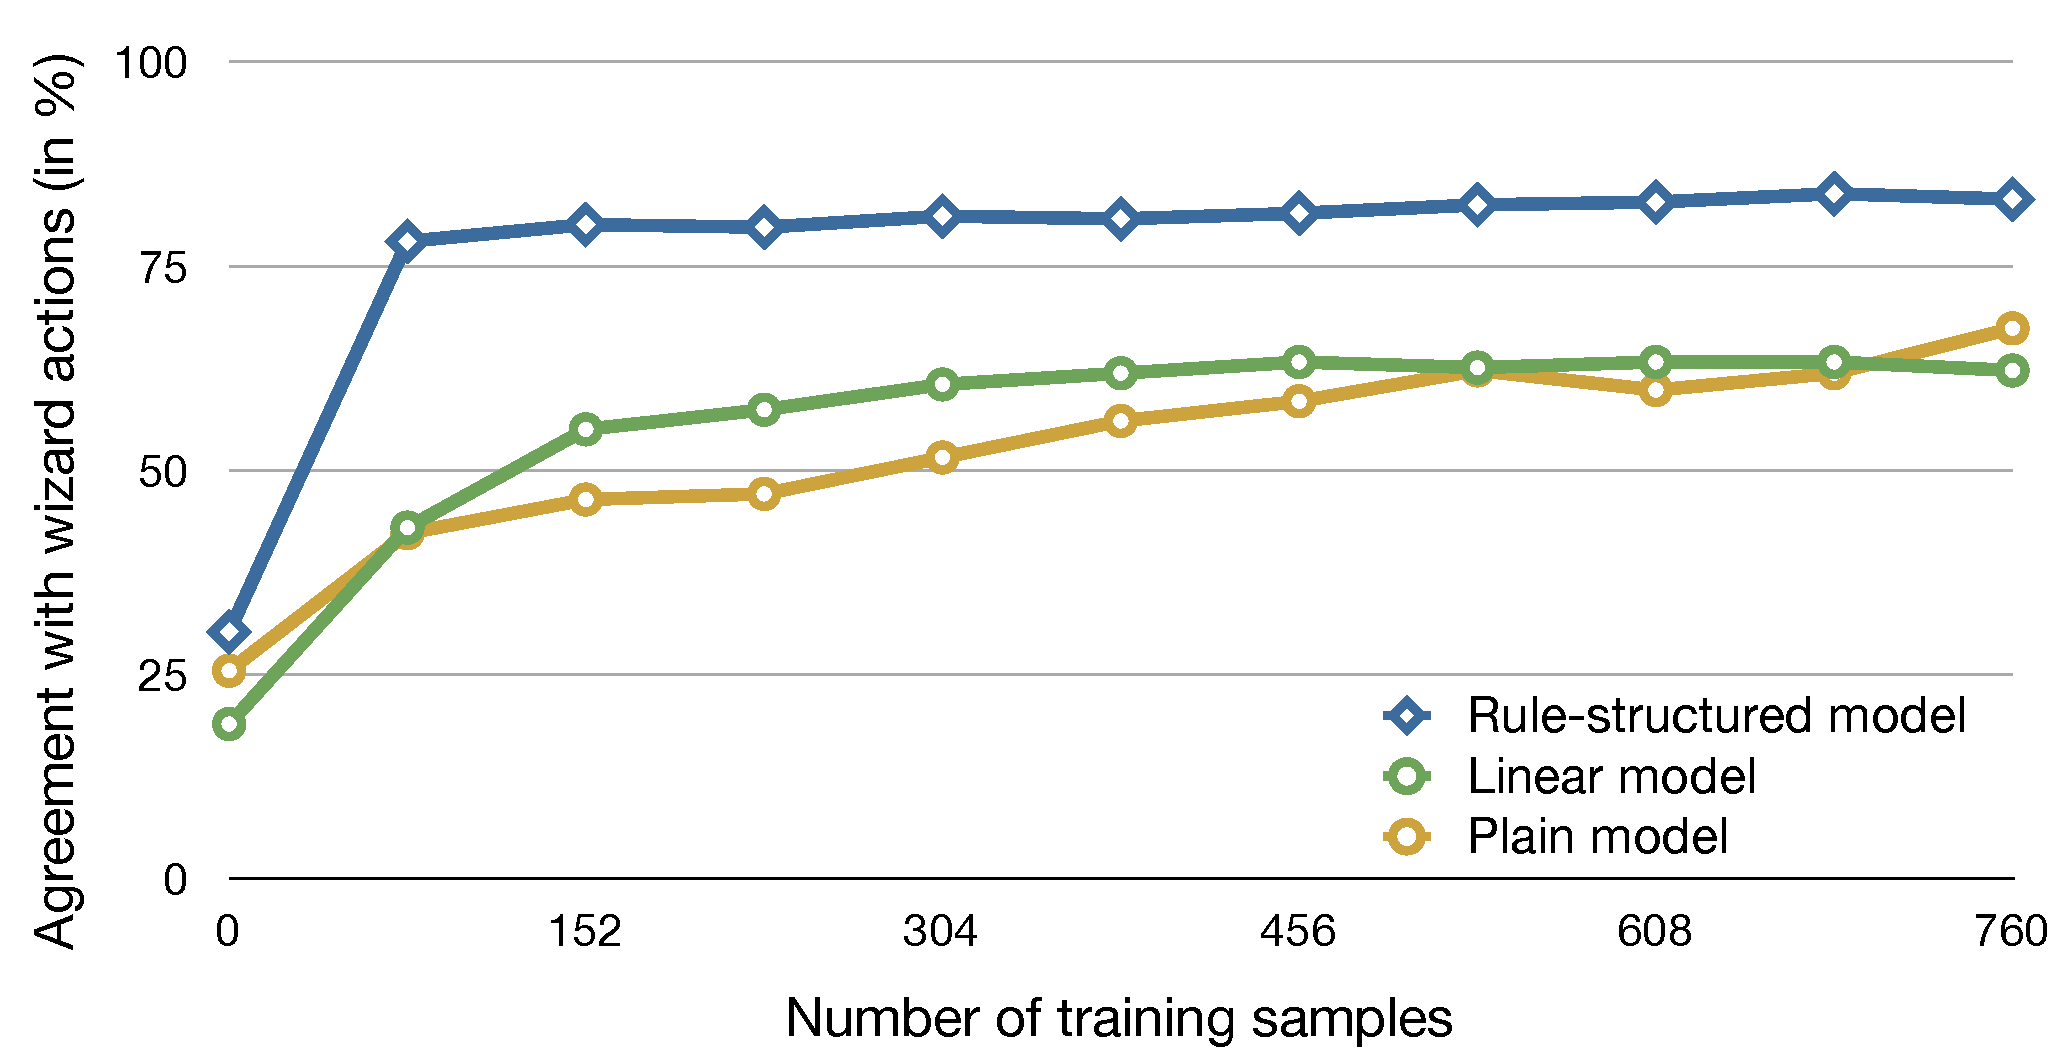
\includegraphics[scale=0.30]{imgs/results_linear.pdf}
\label{subfig:linear_results}
}\end{center} $\phantom{a}$\vspace{1cm}$\phantom{a}$ 
\begin{center}\subfigure[Logarithmic scale (base 2)]{
\centering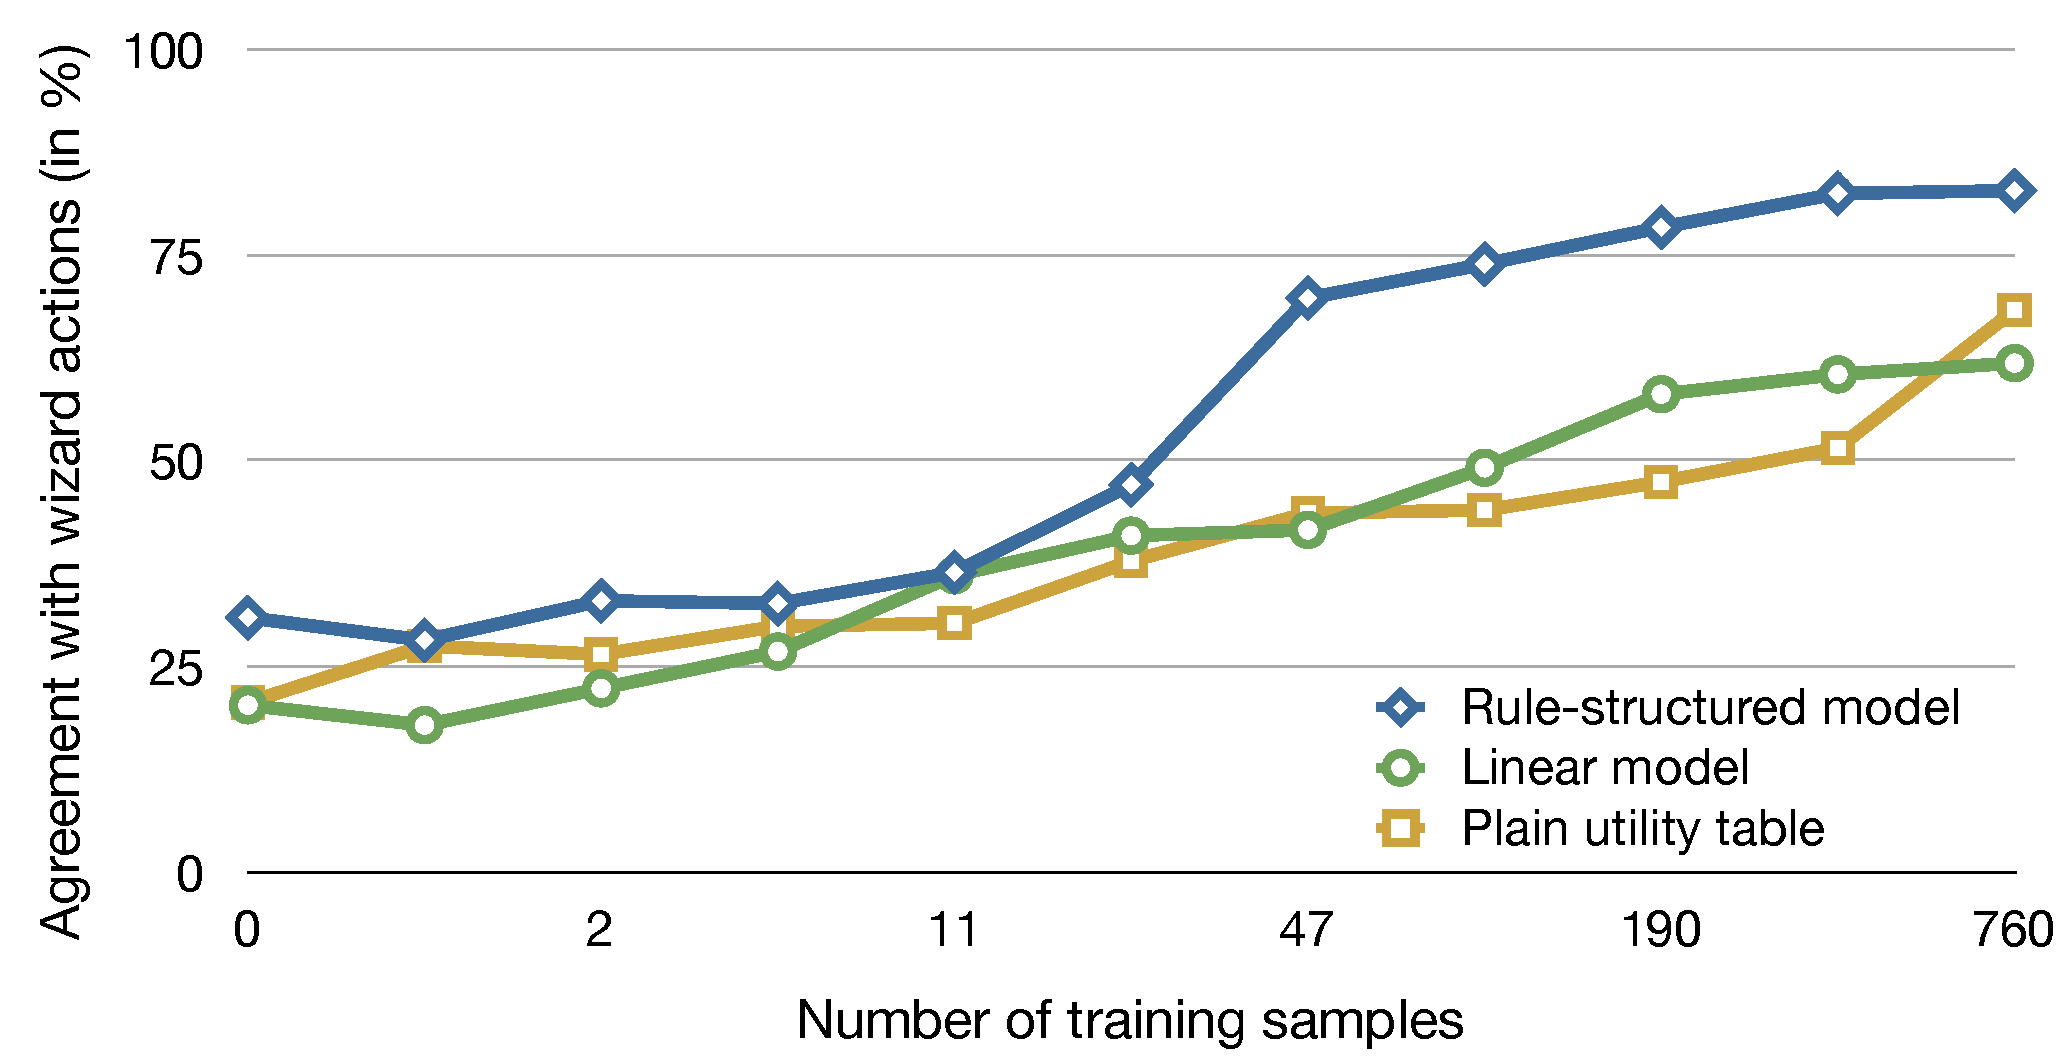
\includegraphics[scale=0.30]{imgs/results_log.pdf}
\label{subfig:exp_results}
}\end{center}
\caption{Learning curves for the learned utility models on a held-out test set of 255 actions as a function of the number of processed data points.  The accuracy results are given for the plain, linear and rule-structured utility models, using both linear (top) and logarithmic scales (bottom).}
\label{results}
\end{figure*}

\section{Conclusion}
\label{sec:woz-conclusions}


We showed in this chapter how to (1) include parameters in the specification of probabilistic rules and (2) use Bayesian learning techniques to automatically estimate these parameters from data.  The rule parameters can represent either utilities or probabilities.  The learning process starts by defining prior distributions over the parameter values and gradually refine these distributions based on the available data points. Multiple parameter priors can be used to this end, such as Dirichlet priors for probability values and Gaussian or uniform priors for utilities. 

The main focus of the chapter was on supervised learning of rule parameters based on training data collected from Wizard-of-Oz interactions. We described how Wizard-of-Oz data can be collected and processed in order to provide data points encoded as pairs <dialogue state $\mathcal{B}_i$, wizard action $a_i$>.  
These data points can be used to progressively narrow down the spread of the posterior distributions over the parameter values to the values that best fit the given data. 

The presented approach has been implemented in a full-fledged spoken dialogue system for human-robot interaction and validated in a simple learning experiment.  The goal of the experiment was to estimate the utility values of various actions on the basis of a Wizard-of-Oz data set.  Three models were compared: a plain utility table, a linear model, and a rule-structured model. The empirical results have shown that the rule structure enables the learning algorithm to converge faster and with better generalisation performance.

Wizard-of-Oz interactions are a useful and interesting source of domain knowledge for the estimation of probabilistic models of dialogue. The collection of Wizard-of-Oz data can however be a tedious process, as it requires:
\begin{enumerate}
\item The availability of an expert (the wizard) that can control the system and provide examples of appropriate behaviour for the domain.
\item The technical setup of a Wizard-of-Oz environment from which the wizard can perceive the user inputs, monitor contextual features, select possible actions to execute, and get all relevant information recorded and stored in a generic format. 
\end{enumerate}

A natural alternative to supervised learning from Wizard-of-Oz data is to let the dialogue system learn the best conversational behaviour via trial-and-error from its own interaction experience (that is, through reinforcement learning), without the reliance on external examples.  The next chapter demonstrates how such strategy can be practically implemented with probabilistic rules. 
